% Options for packages loaded elsewhere
\PassOptionsToPackage{unicode}{hyperref}
\PassOptionsToPackage{hyphens}{url}
\PassOptionsToPackage{dvipsnames,svgnames,x11names}{xcolor}
%
\documentclass[
  letterpaper,
  DIV=11,
  numbers=noendperiod]{scrreprt}

\usepackage{amsmath,amssymb}
\usepackage{iftex}
\ifPDFTeX
  \usepackage[T1]{fontenc}
  \usepackage[utf8]{inputenc}
  \usepackage{textcomp} % provide euro and other symbols
\else % if luatex or xetex
  \usepackage{unicode-math}
  \defaultfontfeatures{Scale=MatchLowercase}
  \defaultfontfeatures[\rmfamily]{Ligatures=TeX,Scale=1}
\fi
\usepackage{lmodern}
\ifPDFTeX\else  
    % xetex/luatex font selection
\fi
% Use upquote if available, for straight quotes in verbatim environments
\IfFileExists{upquote.sty}{\usepackage{upquote}}{}
\IfFileExists{microtype.sty}{% use microtype if available
  \usepackage[]{microtype}
  \UseMicrotypeSet[protrusion]{basicmath} % disable protrusion for tt fonts
}{}
\makeatletter
\@ifundefined{KOMAClassName}{% if non-KOMA class
  \IfFileExists{parskip.sty}{%
    \usepackage{parskip}
  }{% else
    \setlength{\parindent}{0pt}
    \setlength{\parskip}{6pt plus 2pt minus 1pt}}
}{% if KOMA class
  \KOMAoptions{parskip=half}}
\makeatother
\usepackage{xcolor}
\setlength{\emergencystretch}{3em} % prevent overfull lines
\setcounter{secnumdepth}{5}
% Make \paragraph and \subparagraph free-standing
\ifx\paragraph\undefined\else
  \let\oldparagraph\paragraph
  \renewcommand{\paragraph}[1]{\oldparagraph{#1}\mbox{}}
\fi
\ifx\subparagraph\undefined\else
  \let\oldsubparagraph\subparagraph
  \renewcommand{\subparagraph}[1]{\oldsubparagraph{#1}\mbox{}}
\fi

\usepackage{color}
\usepackage{fancyvrb}
\newcommand{\VerbBar}{|}
\newcommand{\VERB}{\Verb[commandchars=\\\{\}]}
\DefineVerbatimEnvironment{Highlighting}{Verbatim}{commandchars=\\\{\}}
% Add ',fontsize=\small' for more characters per line
\usepackage{framed}
\definecolor{shadecolor}{RGB}{241,243,245}
\newenvironment{Shaded}{\begin{snugshade}}{\end{snugshade}}
\newcommand{\AlertTok}[1]{\textcolor[rgb]{0.68,0.00,0.00}{#1}}
\newcommand{\AnnotationTok}[1]{\textcolor[rgb]{0.37,0.37,0.37}{#1}}
\newcommand{\AttributeTok}[1]{\textcolor[rgb]{0.40,0.45,0.13}{#1}}
\newcommand{\BaseNTok}[1]{\textcolor[rgb]{0.68,0.00,0.00}{#1}}
\newcommand{\BuiltInTok}[1]{\textcolor[rgb]{0.00,0.23,0.31}{#1}}
\newcommand{\CharTok}[1]{\textcolor[rgb]{0.13,0.47,0.30}{#1}}
\newcommand{\CommentTok}[1]{\textcolor[rgb]{0.37,0.37,0.37}{#1}}
\newcommand{\CommentVarTok}[1]{\textcolor[rgb]{0.37,0.37,0.37}{\textit{#1}}}
\newcommand{\ConstantTok}[1]{\textcolor[rgb]{0.56,0.35,0.01}{#1}}
\newcommand{\ControlFlowTok}[1]{\textcolor[rgb]{0.00,0.23,0.31}{#1}}
\newcommand{\DataTypeTok}[1]{\textcolor[rgb]{0.68,0.00,0.00}{#1}}
\newcommand{\DecValTok}[1]{\textcolor[rgb]{0.68,0.00,0.00}{#1}}
\newcommand{\DocumentationTok}[1]{\textcolor[rgb]{0.37,0.37,0.37}{\textit{#1}}}
\newcommand{\ErrorTok}[1]{\textcolor[rgb]{0.68,0.00,0.00}{#1}}
\newcommand{\ExtensionTok}[1]{\textcolor[rgb]{0.00,0.23,0.31}{#1}}
\newcommand{\FloatTok}[1]{\textcolor[rgb]{0.68,0.00,0.00}{#1}}
\newcommand{\FunctionTok}[1]{\textcolor[rgb]{0.28,0.35,0.67}{#1}}
\newcommand{\ImportTok}[1]{\textcolor[rgb]{0.00,0.46,0.62}{#1}}
\newcommand{\InformationTok}[1]{\textcolor[rgb]{0.37,0.37,0.37}{#1}}
\newcommand{\KeywordTok}[1]{\textcolor[rgb]{0.00,0.23,0.31}{#1}}
\newcommand{\NormalTok}[1]{\textcolor[rgb]{0.00,0.23,0.31}{#1}}
\newcommand{\OperatorTok}[1]{\textcolor[rgb]{0.37,0.37,0.37}{#1}}
\newcommand{\OtherTok}[1]{\textcolor[rgb]{0.00,0.23,0.31}{#1}}
\newcommand{\PreprocessorTok}[1]{\textcolor[rgb]{0.68,0.00,0.00}{#1}}
\newcommand{\RegionMarkerTok}[1]{\textcolor[rgb]{0.00,0.23,0.31}{#1}}
\newcommand{\SpecialCharTok}[1]{\textcolor[rgb]{0.37,0.37,0.37}{#1}}
\newcommand{\SpecialStringTok}[1]{\textcolor[rgb]{0.13,0.47,0.30}{#1}}
\newcommand{\StringTok}[1]{\textcolor[rgb]{0.13,0.47,0.30}{#1}}
\newcommand{\VariableTok}[1]{\textcolor[rgb]{0.07,0.07,0.07}{#1}}
\newcommand{\VerbatimStringTok}[1]{\textcolor[rgb]{0.13,0.47,0.30}{#1}}
\newcommand{\WarningTok}[1]{\textcolor[rgb]{0.37,0.37,0.37}{\textit{#1}}}

\providecommand{\tightlist}{%
  \setlength{\itemsep}{0pt}\setlength{\parskip}{0pt}}\usepackage{longtable,booktabs,array}
\usepackage{calc} % for calculating minipage widths
% Correct order of tables after \paragraph or \subparagraph
\usepackage{etoolbox}
\makeatletter
\patchcmd\longtable{\par}{\if@noskipsec\mbox{}\fi\par}{}{}
\makeatother
% Allow footnotes in longtable head/foot
\IfFileExists{footnotehyper.sty}{\usepackage{footnotehyper}}{\usepackage{footnote}}
\makesavenoteenv{longtable}
\usepackage{graphicx}
\makeatletter
\def\maxwidth{\ifdim\Gin@nat@width>\linewidth\linewidth\else\Gin@nat@width\fi}
\def\maxheight{\ifdim\Gin@nat@height>\textheight\textheight\else\Gin@nat@height\fi}
\makeatother
% Scale images if necessary, so that they will not overflow the page
% margins by default, and it is still possible to overwrite the defaults
% using explicit options in \includegraphics[width, height, ...]{}
\setkeys{Gin}{width=\maxwidth,height=\maxheight,keepaspectratio}
% Set default figure placement to htbp
\makeatletter
\def\fps@figure{htbp}
\makeatother
\newlength{\cslhangindent}
\setlength{\cslhangindent}{1.5em}
\newlength{\csllabelwidth}
\setlength{\csllabelwidth}{3em}
\newlength{\cslentryspacingunit} % times entry-spacing
\setlength{\cslentryspacingunit}{\parskip}
\newenvironment{CSLReferences}[2] % #1 hanging-ident, #2 entry spacing
 {% don't indent paragraphs
  \setlength{\parindent}{0pt}
  % turn on hanging indent if param 1 is 1
  \ifodd #1
  \let\oldpar\par
  \def\par{\hangindent=\cslhangindent\oldpar}
  \fi
  % set entry spacing
  \setlength{\parskip}{#2\cslentryspacingunit}
 }%
 {}
\usepackage{calc}
\newcommand{\CSLBlock}[1]{#1\hfill\break}
\newcommand{\CSLLeftMargin}[1]{\parbox[t]{\csllabelwidth}{#1}}
\newcommand{\CSLRightInline}[1]{\parbox[t]{\linewidth - \csllabelwidth}{#1}\break}
\newcommand{\CSLIndent}[1]{\hspace{\cslhangindent}#1}

\KOMAoption{captions}{tableheading}
\makeatletter
\@ifpackageloaded{tcolorbox}{}{\usepackage[skins,breakable]{tcolorbox}}
\@ifpackageloaded{fontawesome5}{}{\usepackage{fontawesome5}}
\definecolor{quarto-callout-color}{HTML}{909090}
\definecolor{quarto-callout-note-color}{HTML}{0758E5}
\definecolor{quarto-callout-important-color}{HTML}{CC1914}
\definecolor{quarto-callout-warning-color}{HTML}{EB9113}
\definecolor{quarto-callout-tip-color}{HTML}{00A047}
\definecolor{quarto-callout-caution-color}{HTML}{FC5300}
\definecolor{quarto-callout-color-frame}{HTML}{acacac}
\definecolor{quarto-callout-note-color-frame}{HTML}{4582ec}
\definecolor{quarto-callout-important-color-frame}{HTML}{d9534f}
\definecolor{quarto-callout-warning-color-frame}{HTML}{f0ad4e}
\definecolor{quarto-callout-tip-color-frame}{HTML}{02b875}
\definecolor{quarto-callout-caution-color-frame}{HTML}{fd7e14}
\makeatother
\makeatletter
\makeatother
\makeatletter
\@ifpackageloaded{bookmark}{}{\usepackage{bookmark}}
\makeatother
\makeatletter
\@ifpackageloaded{caption}{}{\usepackage{caption}}
\AtBeginDocument{%
\ifdefined\contentsname
  \renewcommand*\contentsname{Table of contents}
\else
  \newcommand\contentsname{Table of contents}
\fi
\ifdefined\listfigurename
  \renewcommand*\listfigurename{List of Figures}
\else
  \newcommand\listfigurename{List of Figures}
\fi
\ifdefined\listtablename
  \renewcommand*\listtablename{List of Tables}
\else
  \newcommand\listtablename{List of Tables}
\fi
\ifdefined\figurename
  \renewcommand*\figurename{Figure}
\else
  \newcommand\figurename{Figure}
\fi
\ifdefined\tablename
  \renewcommand*\tablename{Table}
\else
  \newcommand\tablename{Table}
\fi
}
\@ifpackageloaded{float}{}{\usepackage{float}}
\floatstyle{ruled}
\@ifundefined{c@chapter}{\newfloat{codelisting}{h}{lop}}{\newfloat{codelisting}{h}{lop}[chapter]}
\floatname{codelisting}{Listing}
\newcommand*\listoflistings{\listof{codelisting}{List of Listings}}
\makeatother
\makeatletter
\@ifpackageloaded{caption}{}{\usepackage{caption}}
\@ifpackageloaded{subcaption}{}{\usepackage{subcaption}}
\makeatother
\makeatletter
\@ifpackageloaded{tcolorbox}{}{\usepackage[skins,breakable]{tcolorbox}}
\makeatother
\makeatletter
\@ifundefined{shadecolor}{\definecolor{shadecolor}{rgb}{.97, .97, .97}}
\makeatother
\makeatletter
\makeatother
\makeatletter
\makeatother
\ifLuaTeX
  \usepackage{selnolig}  % disable illegal ligatures
\fi
\IfFileExists{bookmark.sty}{\usepackage{bookmark}}{\usepackage{hyperref}}
\IfFileExists{xurl.sty}{\usepackage{xurl}}{} % add URL line breaks if available
\urlstyle{same} % disable monospaced font for URLs
\hypersetup{
  pdftitle={antibioticsbook},
  pdfauthor={Russell Lewis},
  colorlinks=true,
  linkcolor={blue},
  filecolor={Maroon},
  citecolor={Blue},
  urlcolor={Blue},
  pdfcreator={LaTeX via pandoc}}

\title{antibioticsbook}
\author{Russell Lewis}
\date{2023-07-25}

\begin{document}
\maketitle
\ifdefined\Shaded\renewenvironment{Shaded}{\begin{tcolorbox}[sharp corners, enhanced, frame hidden, boxrule=0pt, breakable, borderline west={3pt}{0pt}{shadecolor}, interior hidden]}{\end{tcolorbox}}\fi

\renewcommand*\contentsname{Table of contents}
{
\hypersetup{linkcolor=}
\setcounter{tocdepth}{2}
\tableofcontents
}
\bookmarksetup{startatroot}

\hypertarget{preface}{%
\chapter*{Preface}\label{preface}}
\addcontentsline{toc}{chapter}{Preface}

\markboth{Preface}{Preface}

This is a Quarto book.

To learn more about Quarto books visit
\url{https://quarto.org/docs/books}.

\bookmarksetup{startatroot}

\hypertarget{antibiotic-testing-in-the-laboratory}{%
\chapter{Antibiotic testing in the
laboratory}\label{antibiotic-testing-in-the-laboratory}}

\bookmarksetup{startatroot}

\hypertarget{history-of-antibiotic-development}{%
\chapter{History of Antibiotic
Development}\label{history-of-antibiotic-development}}

\begin{tcolorbox}[enhanced jigsaw, toptitle=1mm, colframe=quarto-callout-note-color-frame, arc=.35mm, rightrule=.15mm, title=\textcolor{quarto-callout-note-color}{\faInfo}\hspace{0.5em}{Learning objectives}, leftrule=.75mm, opacityback=0, opacitybacktitle=0.6, breakable, coltitle=black, toprule=.15mm, colback=white, colbacktitle=quarto-callout-note-color!10!white, bottomtitle=1mm, titlerule=0mm, bottomrule=.15mm, left=2mm]

\begin{itemize}
\item
  Compare and contrast natural, semisynthetic, and synthetic
  antimicrobial drugs
\item
  Describe the historically important individuals and events that led to
  the development of antimicrobial drugs
\item
  Identify the key challenges in development of future antibiotics
\end{itemize}

\end{tcolorbox}

\hypertarget{the-impact-of-antibiotics-on-human-health}{%
\section*{The impact of antibiotics on human
health}\label{the-impact-of-antibiotics-on-human-health}}
\addcontentsline{toc}{section}{The impact of antibiotics on human
health}

\markright{The impact of antibiotics on human health}

Until the 20th Century, influenza, pneumonia, tuberculosis, and enteric
infections ranked among the leading causes of death. The average
lifespan for adults in Western Europe was around 50 years, with a 2\%
mortality rate for children under the age of 5 due to premature deaths
primarily caused by infectious diseases.

Industrialization and increasing wealth during the 19th century brought
improvements in drinking water and sanitation in many countries, leading
to reductions in communicable enteric infections and improved in life
expectancy Figure~\ref{fig-lifeexp}. By the early 20th century, vaccines
for pertussis, diphtheria, yellow fever and tuberculosis were
introduced. However, common bacterial infections remained a serious
medical threat. Streptococcal throat infections were sometimes fatal,
ear infections could progress to deafness, mastoiditis or meningitis.
Minor surgeries were associated with risk of life-threatening
infections. Maternal mortality during childbirth approached 2\%.

\begin{figure}

{\centering 

}

\caption{\label{fig-lifeexp}Changes in life expectancy over 500 years.
Source: World in Data}

\end{figure}

The introduction of effective antibiotic therapy played a crucial role
in further reducing mortality rates associated with common infectious
diseases. This breakthrough not only improved the safety of childbirth
and common surgical procedures but also paved the way for supportive
care during chemotherapy for cancer and transplantation. \textbf{Thus
the discovery of antibiotics can be considered one of the most
significant health-related events of modern times.}(Davies and Davies
2010)

\begin{figure}

{\centering 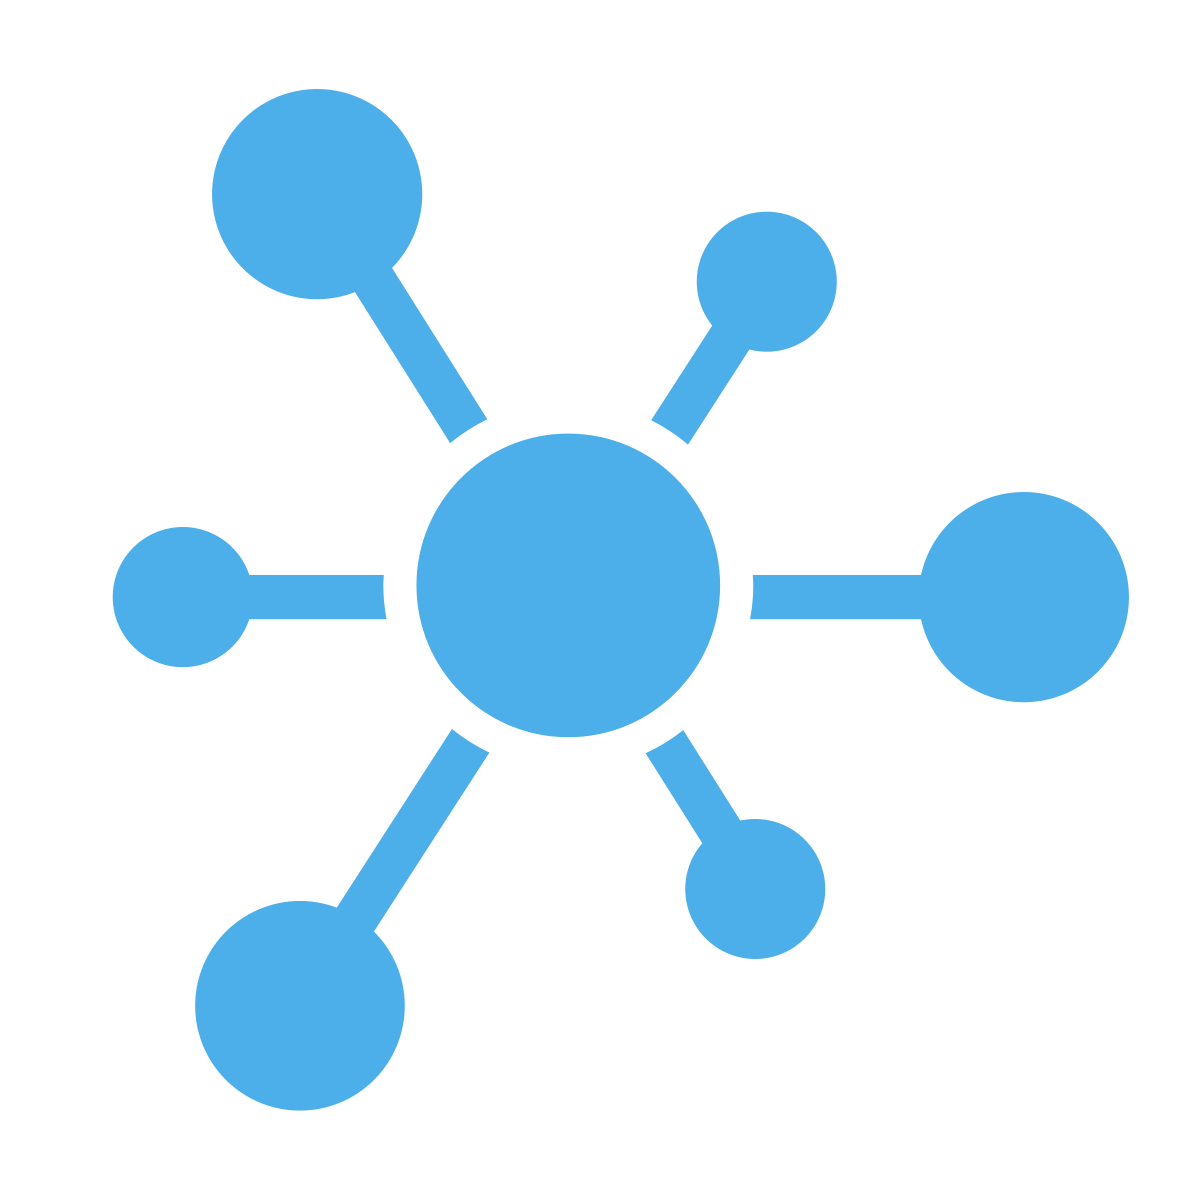
\includegraphics[width=1.04167in,height=\textheight]{images/breakblue.png}

}

\end{figure}

\hypertarget{ancient-use-of-antibiotics}{%
\subsection{Ancient use of
antibiotics}\label{ancient-use-of-antibiotics}}

In nature, some microbes, plants and animals have the ability to produce
substances that can inhibit or kill microbes that cause disease or
compete for the same resources. These natural products have been the
source of many antibiotics and treatments with antimicrobial-like
activity over the millennia.

The first recorded use of antimicrobial -like substances was by the
early Egyptians, Greeks, and Chinese, who used natural products with
antimicrobial activity for millennia to treat wounds and infections,
even if the causes of these diseases were unknown until the 19th and
20th century (Figure~\ref{fig-ancient}). Healers of many cultures
understood the antimicrobial properties of fungi and their use of moldy
bread or other mold-containing products to treat wounds has been well
documented for centuries.(Wainwright 1989) Today, while about 80\% of
the world's population still relies on plant-derived medicines,(Verma
and Singh 2008) scientists are now discovering the active compounds
conferring the medicinal benefits contained in many of these
traditionally used plants.

\begin{figure}

{\centering 

\begin{figure}

{\centering 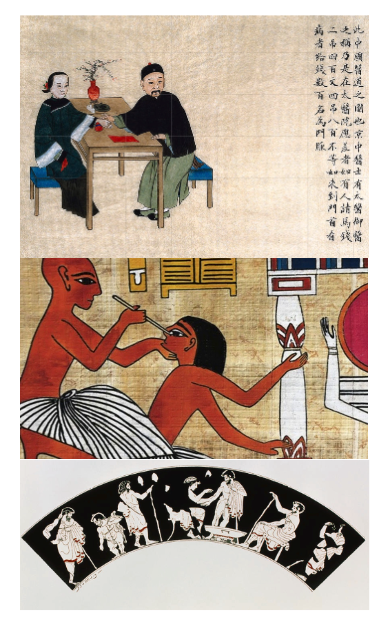
\includegraphics[width=3.125in,height=\textheight]{images/ancient.png}

}

\end{figure}

}

\caption{\label{fig-ancient}Recorded use of antimicrobial-like
treatments by Chinese (top panel), Egyptians (middle) and Greeks (lower
panel). Source: Wikipedia.}

\end{figure}

However, even today some of the most effective anti-infective treatments
(e.g.~artemisinin, which are derivatives from ``qinghao'' or Sweet
Wormwood plant) have been ``rediscovered'' as effective treatments for
severe infectious diseases such as malaria (Figure~\ref{fig-chinese}).

\begin{figure}

{\centering 

\begin{figure}

{\centering 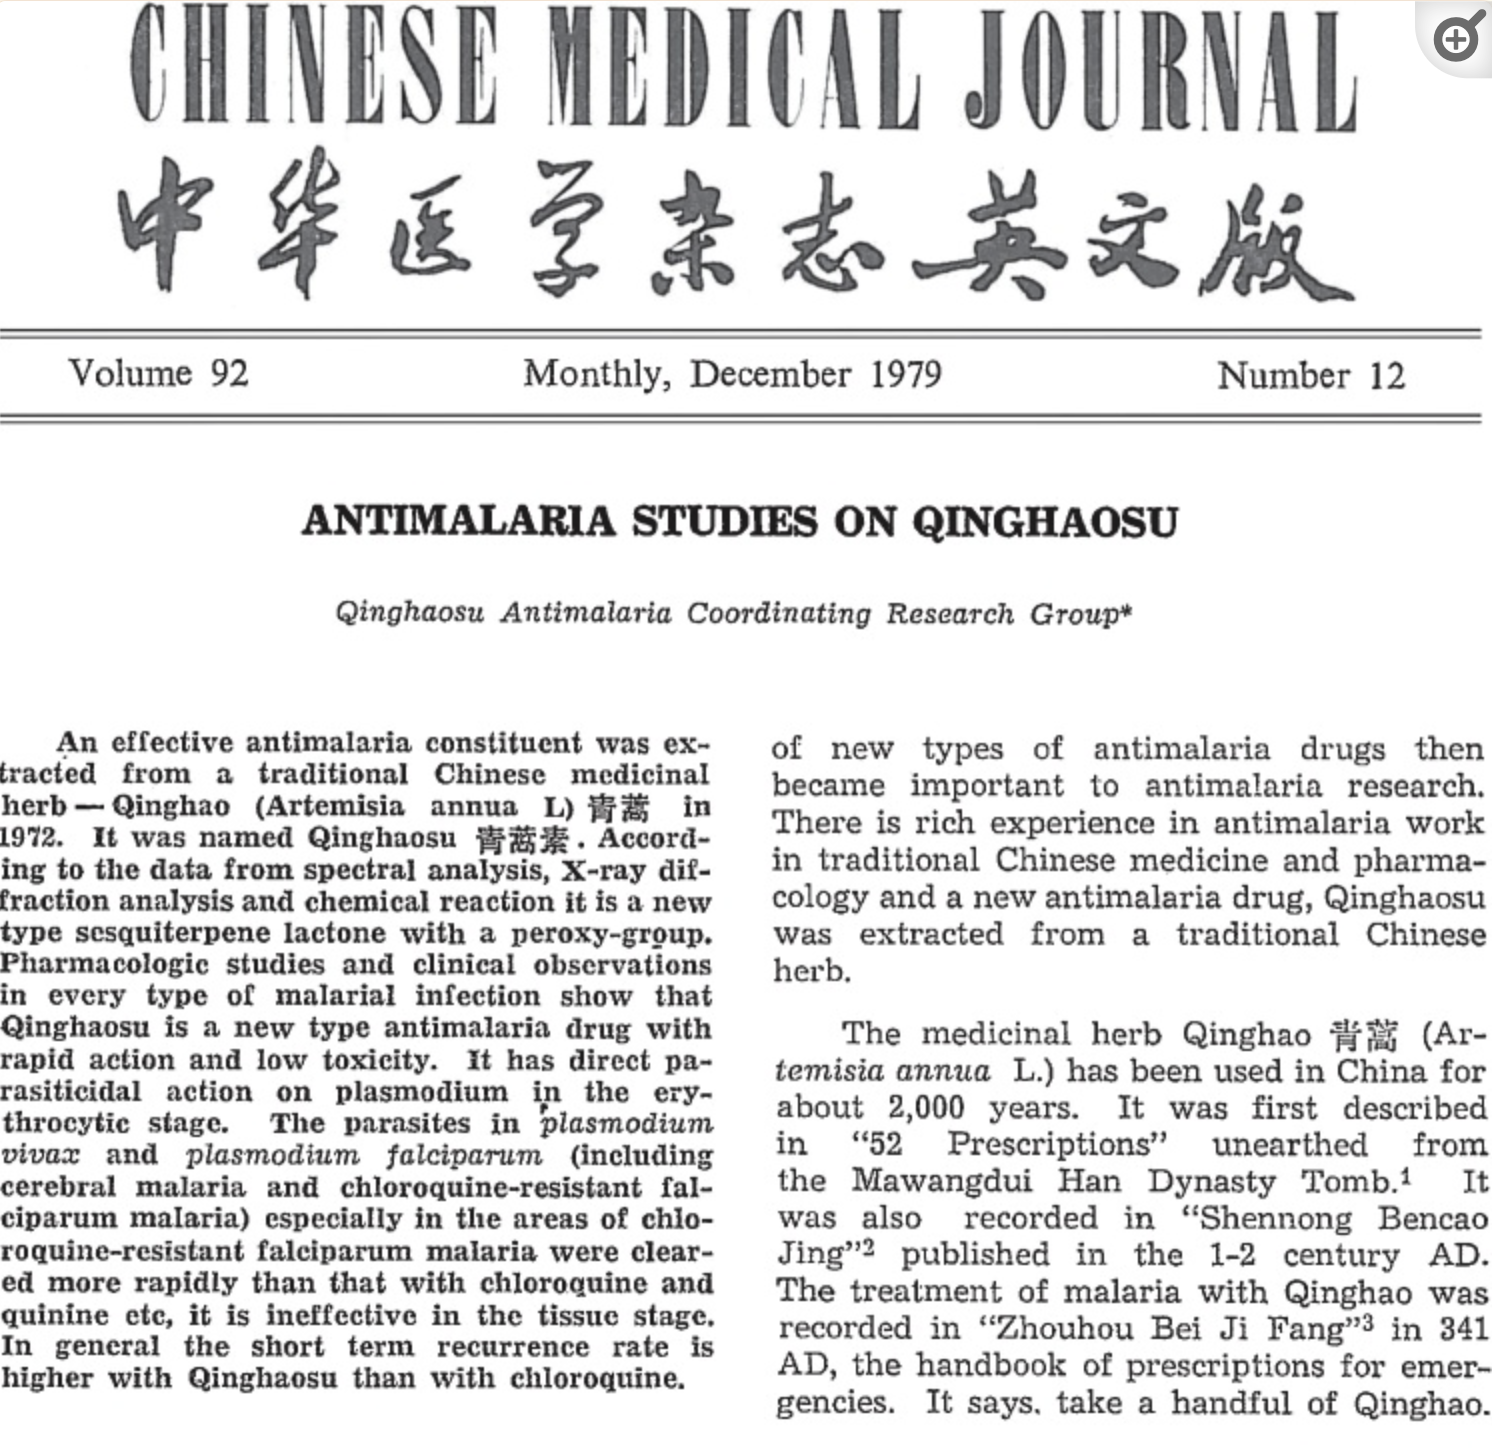
\includegraphics[width=5.20833in,height=\textheight]{images/chinese.png}

}

\end{figure}

}

\caption{\label{fig-chinese}First English-language report of
anti-malarial activity of the artemisinins-a traditional Chinese herbal
remedy. Artemisinins are now the WHO-recommended front-line treatment
for malaria. image course: Chinese Medical Journal}

\end{figure}

Similarly, antibacterial resistance pre-dates the medical use of
antibiotics and is estimated to have emerged with bacteria on earth
approximately 2-2.5 billion years ago. In contrast, the first humans are
believed to have existed around 2 million years ago. Therefore,
antibiotic resistance was not created by humans and misuse of
antibiotics. \textbf{Antibiotic resistance can be considered a biologic
certainty and evolutionary destiny.}

\begin{figure}

{\centering 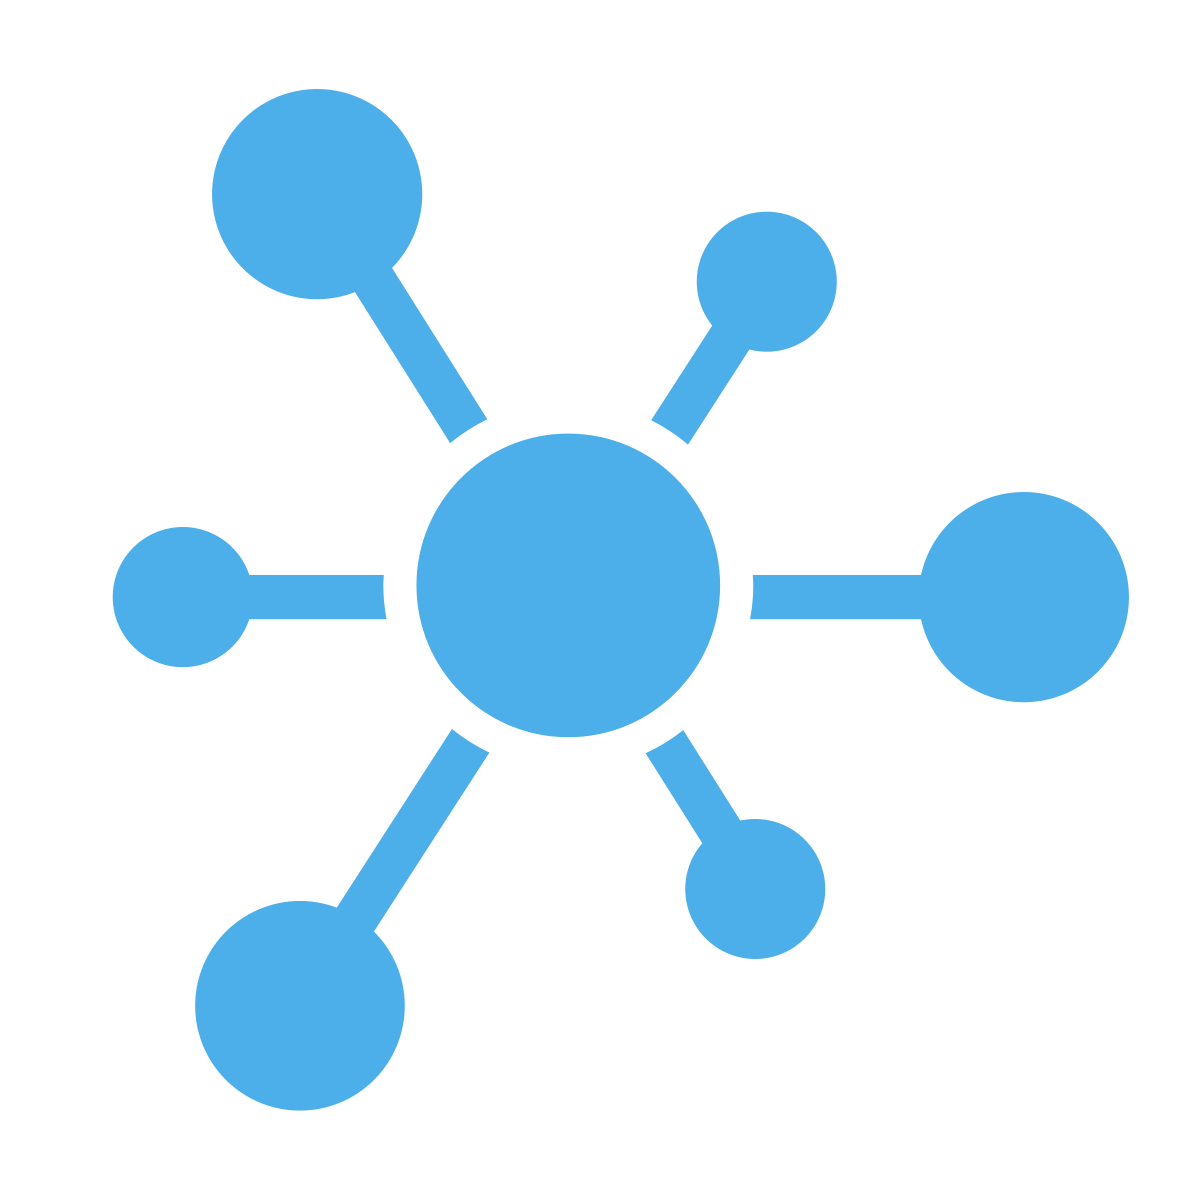
\includegraphics[width=1.04167in,height=\textheight]{images/breakblue.png}

}

\end{figure}

\hypertarget{the-modern-era-of-antibiotic-discovery}{%
\subsection{The modern era of antibiotic
discovery}\label{the-modern-era-of-antibiotic-discovery}}

The microbiologist and immunologist Paul Ehrlich (1854-1915)
(Figure~\ref{fig-paulerlich}) is credited with introduction of
\emph{strategic antibiotic discovery} that with the chemist Sahachiro
Hato lead to the discovery and first medical application of the
synthetic antibiotic arsphenamine (Salvarsan) for the treatment of a
bacterial infection-syphilis. He was awarded the Nobel Prize in Medicine
in 1909.

\begin{figure}

{\centering 

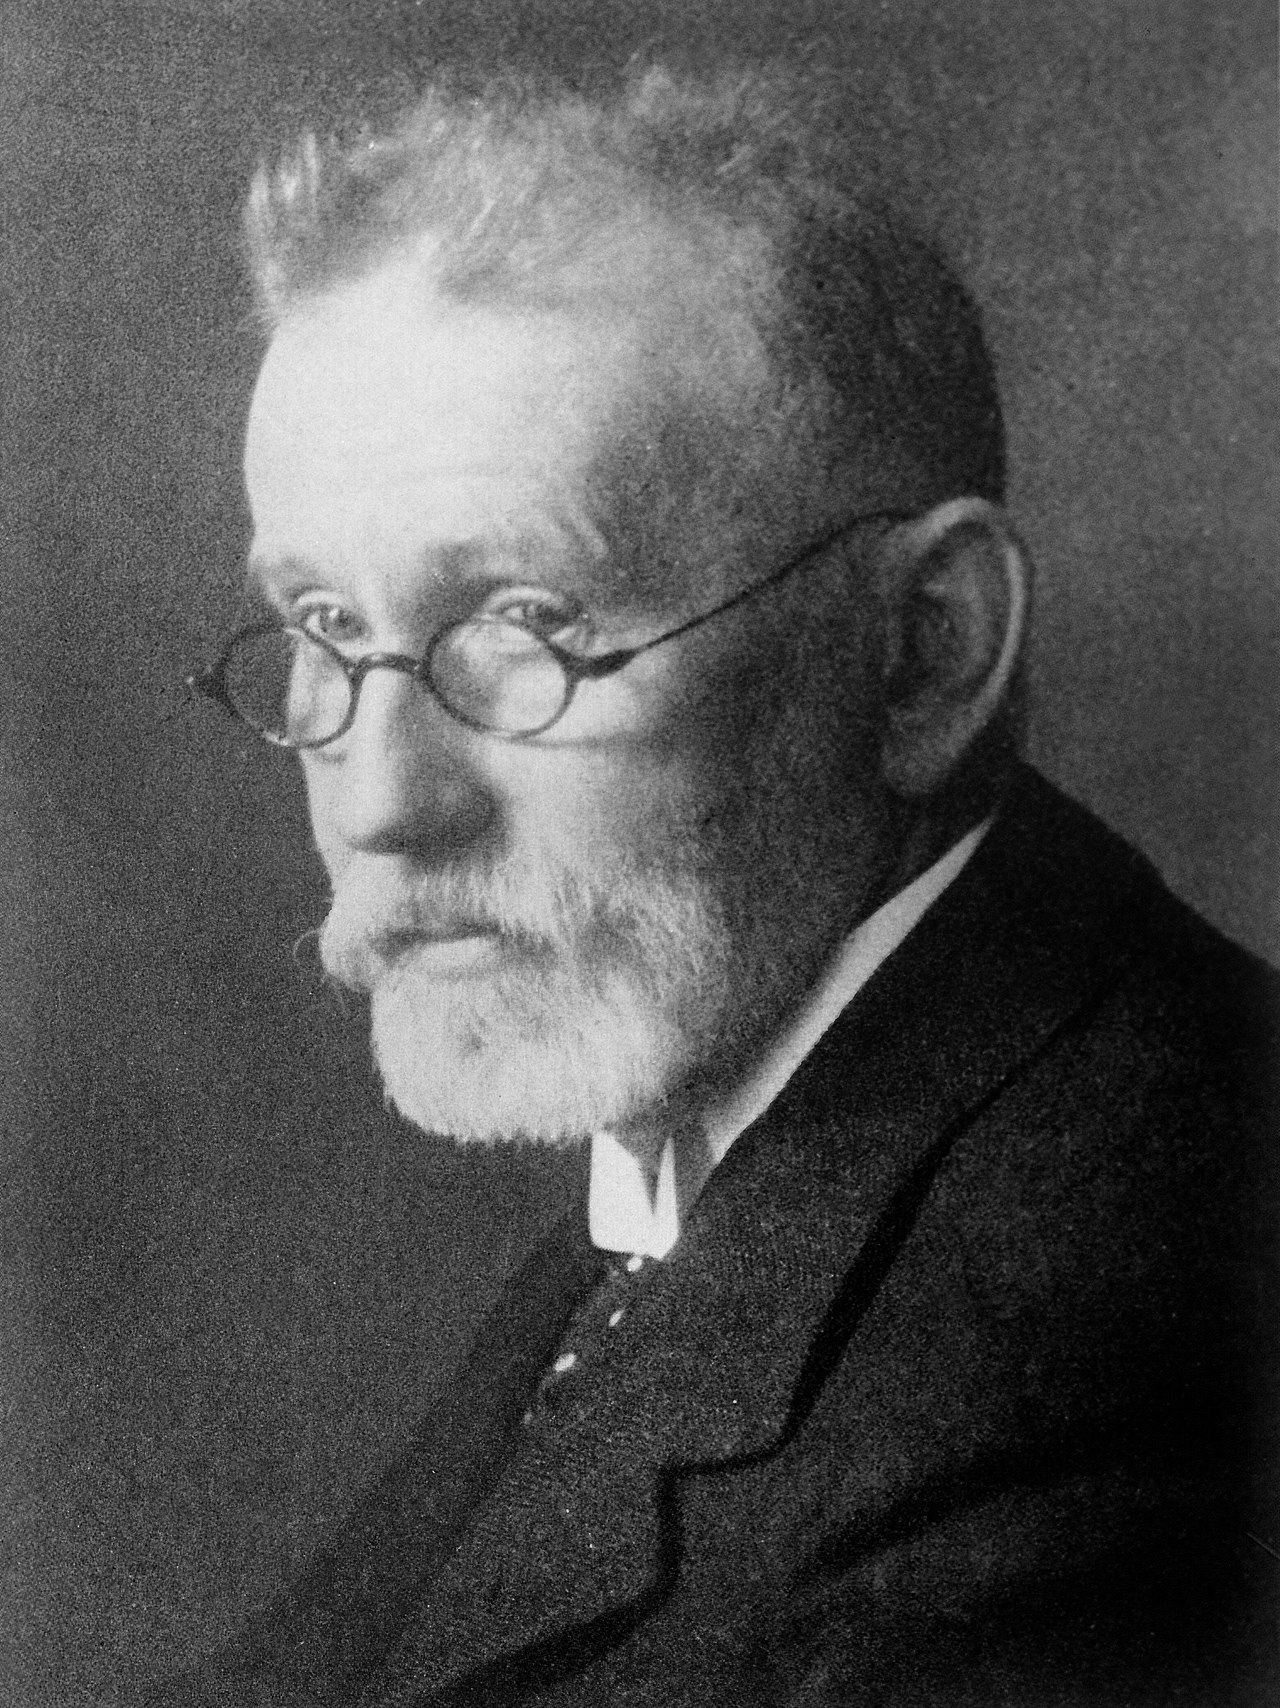
\includegraphics[width=2.60417in,height=\textheight]{images/Paul_Ehrlich_1915.jpg}

}

\caption{\label{fig-paulerlich}German immunologist Paul Ehrlich
(1854-1915). Image: Library of Congress}

\end{figure}

A few decades later, German scientists Josef Klarer, Fritz Mietzsch, and
Gerhard Domagk made a significant discovery regarding the antibacterial
properties of a synthetic dye called \textbf{prontosil}
(Figure~\ref{fig-domagk}). They found that it could effectively treat
streptococcal and staphylococcal infections in mice. Domagk's own
daughter was one of the first individuals to receive the drug, which
successfully cured her severe streptococcal infection caused by a needle
jab. Utterly desperate when the doctor recommended amputation to save
his daughter's life, Domagk treated Hildegard with Prontosil, which led
to her recovery but she suffered a permanent reddish discoloration of
her skin owing to the drug.

In recognition of his work with prontosil and sulfanilamide (the active
compound derived from prontosil), Domagk was awarded the Nobel Prize in
Medicine in 1939. However, the Nobel committee had angered the German
political authorities by awarding the 1935 Nobel Peace Prize to Carl von
Ossietzky, an outspoken German pacifist. Under the grip of Hitler and
the Nazi Party, German citizens were forbidden to accept the Nobel
Prize. After Domagk accepted the prize, he was arrested by the Gestapo
and forced to send a letter rejecting it. Although Domagk was able to
receive his prize medal in 1947, the prize money had long since been
redistributed.

\begin{figure}

{\centering 

\begin{figure}

{\centering 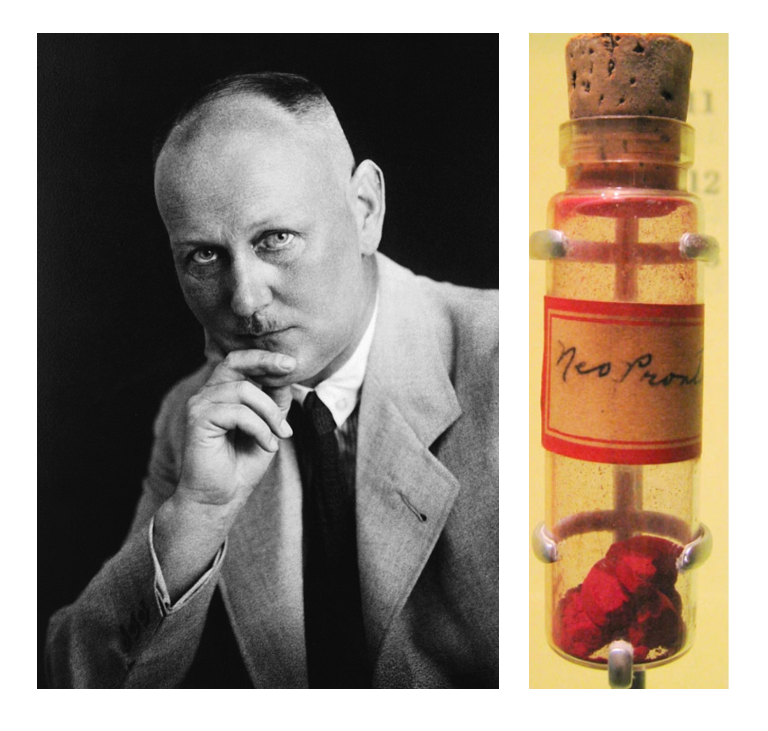
\includegraphics[width=3.125in,height=\textheight]{images/domagk.png}

}

\end{figure}

}

\caption{\label{fig-domagk}Gerhard Domagk (left) and a vial of prontosil
(right), the precursor to sulfanilamide antibiotics}

\end{figure}

Sulfanilamide, the first synthetic antimicrobial, served as the
foundation for the development of a family of sulfa drugs. These
successes led to the discovery and production of other important classes
of synthetic antimicrobials, such as quinolines and oxazolidinones.

\hypertarget{the-discovery-of-penicillin}{%
\subsection{The discovery of
penicillin}\label{the-discovery-of-penicillin}}

A few years prior to the prontosil discovery, Alexander Fleming made an
accidental but ground breaking finding. In 1928, while examining old
plates of staphylococci in his laboratory, Fleming noticed that mold
growth (later identified as \emph{Penicillium notatum}) inhibited the
growth of staphylococci on one plate (Figure~\ref{fig-pcndisc}). This
marked the discovery of penicillin, the first natural antibiotic.
Further experiments carried out by Chain and Florey demonstrated
penicillin's antibacterial properties against streptococci,
meningococci, and \emph{Corynebacterium diphtheriae}, the causative
agent of diphtheria.

While Fleming and his colleagues were credited with the discovery and
identification of penicillin, its isolation and mass production were
achieved by a team of researchers at Oxford University led by Howard
Florey and Ernst Chain. In 1940, they purified penicillin and reported
its success as an antimicrobial agent against streptococcal infections
in mice. Subsequent studies with human subjects also proved penicillin's
effectiveness. For their significant contributions, Fleming, Florey, and
Chain were awarded the Nobel Prize in Physiology and Medicine in 1945.

\begin{figure}

{\centering 

\begin{figure}

{\centering 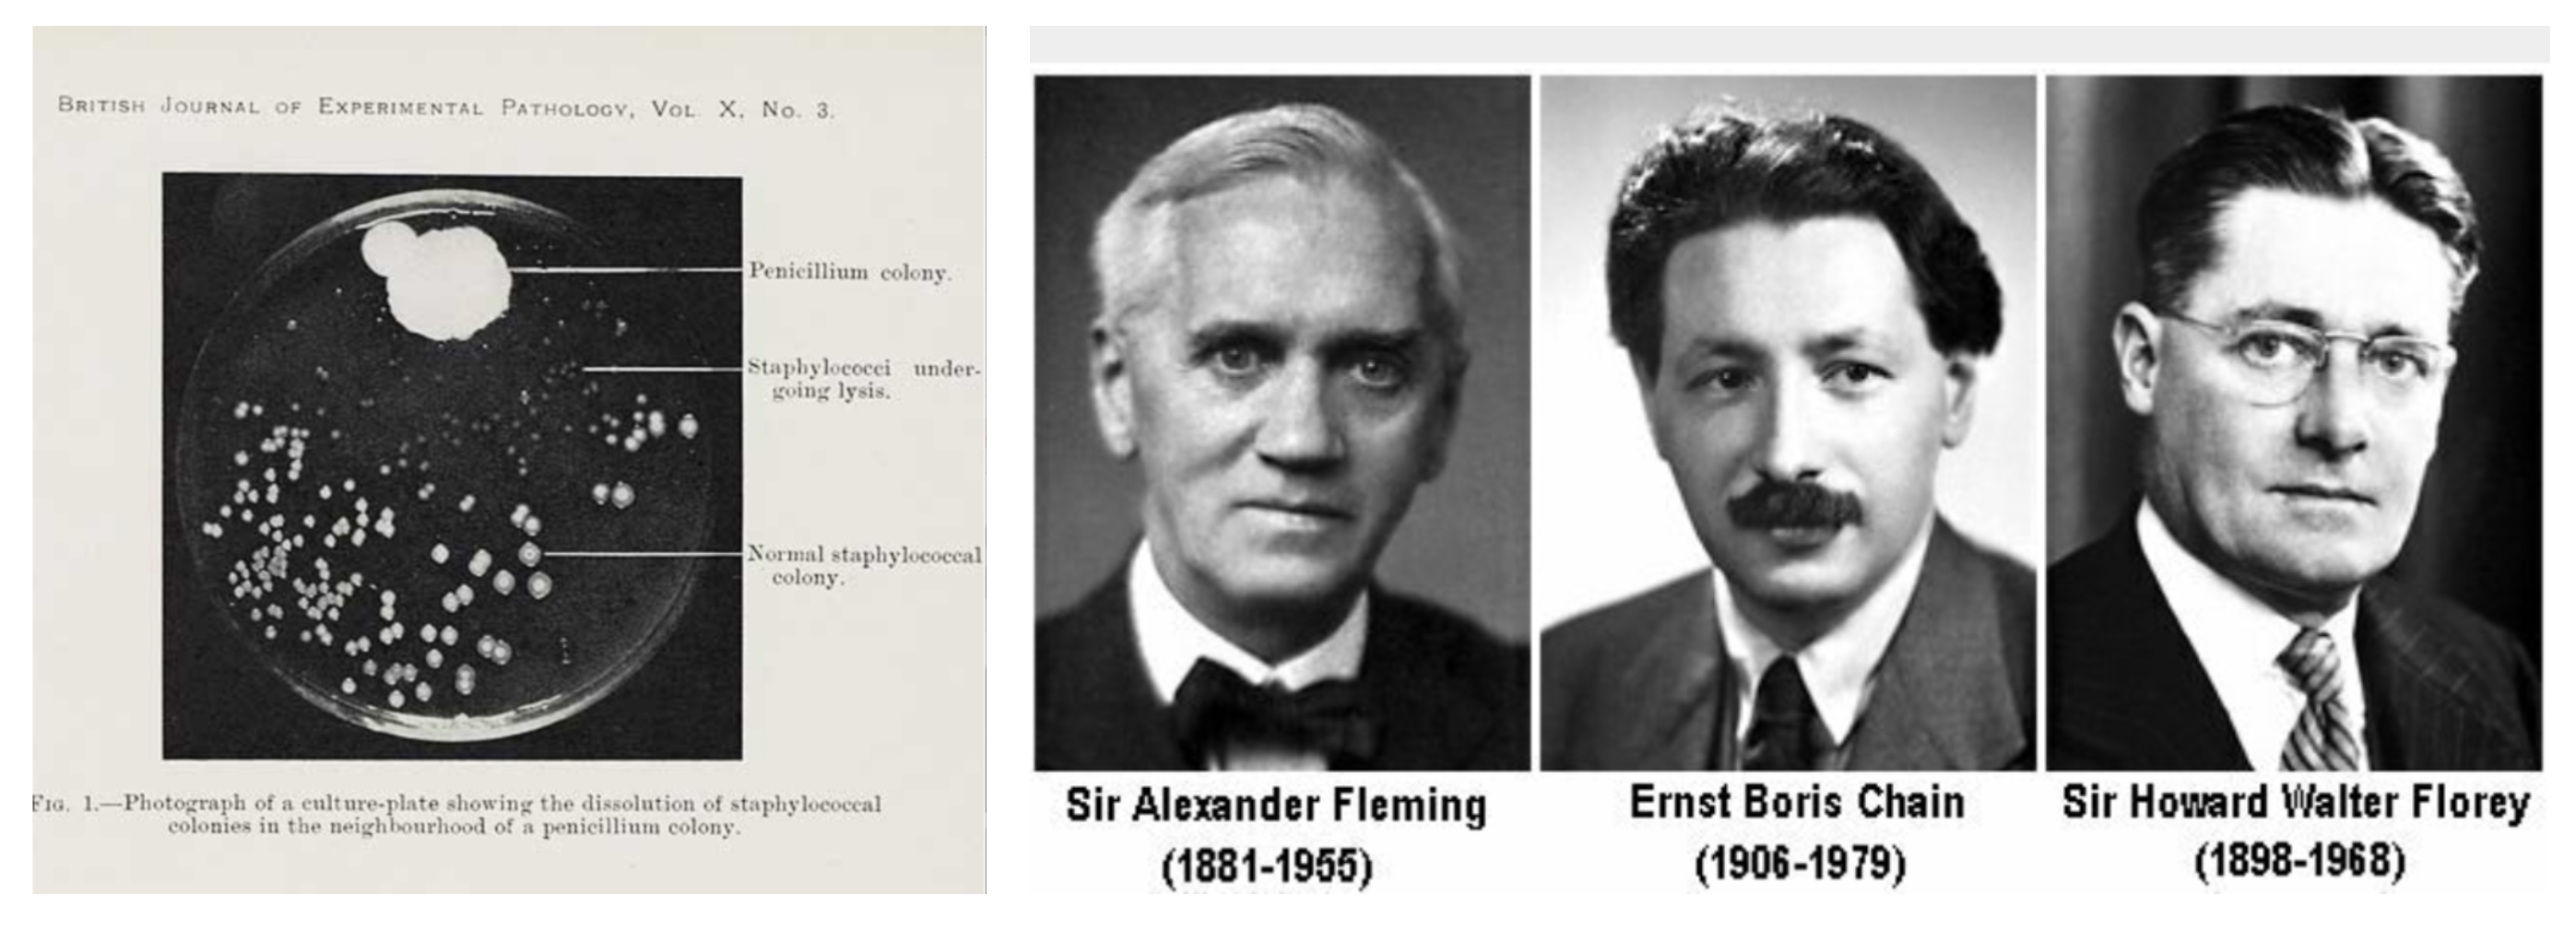
\includegraphics{images/pcndisc.png}

}

\end{figure}

}

\caption{\label{fig-pcndisc}Original report of penicillin antimicrobial
activity in the British Journal of Pathology 1928. The discovers and
developers of penicillin.}

\end{figure}

In June of 1943 Mary Hunt, a lab assistant working in Peoria, Illinois,
found a cantaloupe at a local market covered in mold with a ``pretty,
golden look.'' (Figure~\ref{fig-moldymarry}). This mold turned out to be
a highly productive strain of \emph{Penicillium chrysogeum} and its
discovery marked a turning point in the quest to mass produce
penicillin.

\begin{figure}

{\centering 

\begin{figure}

{\centering 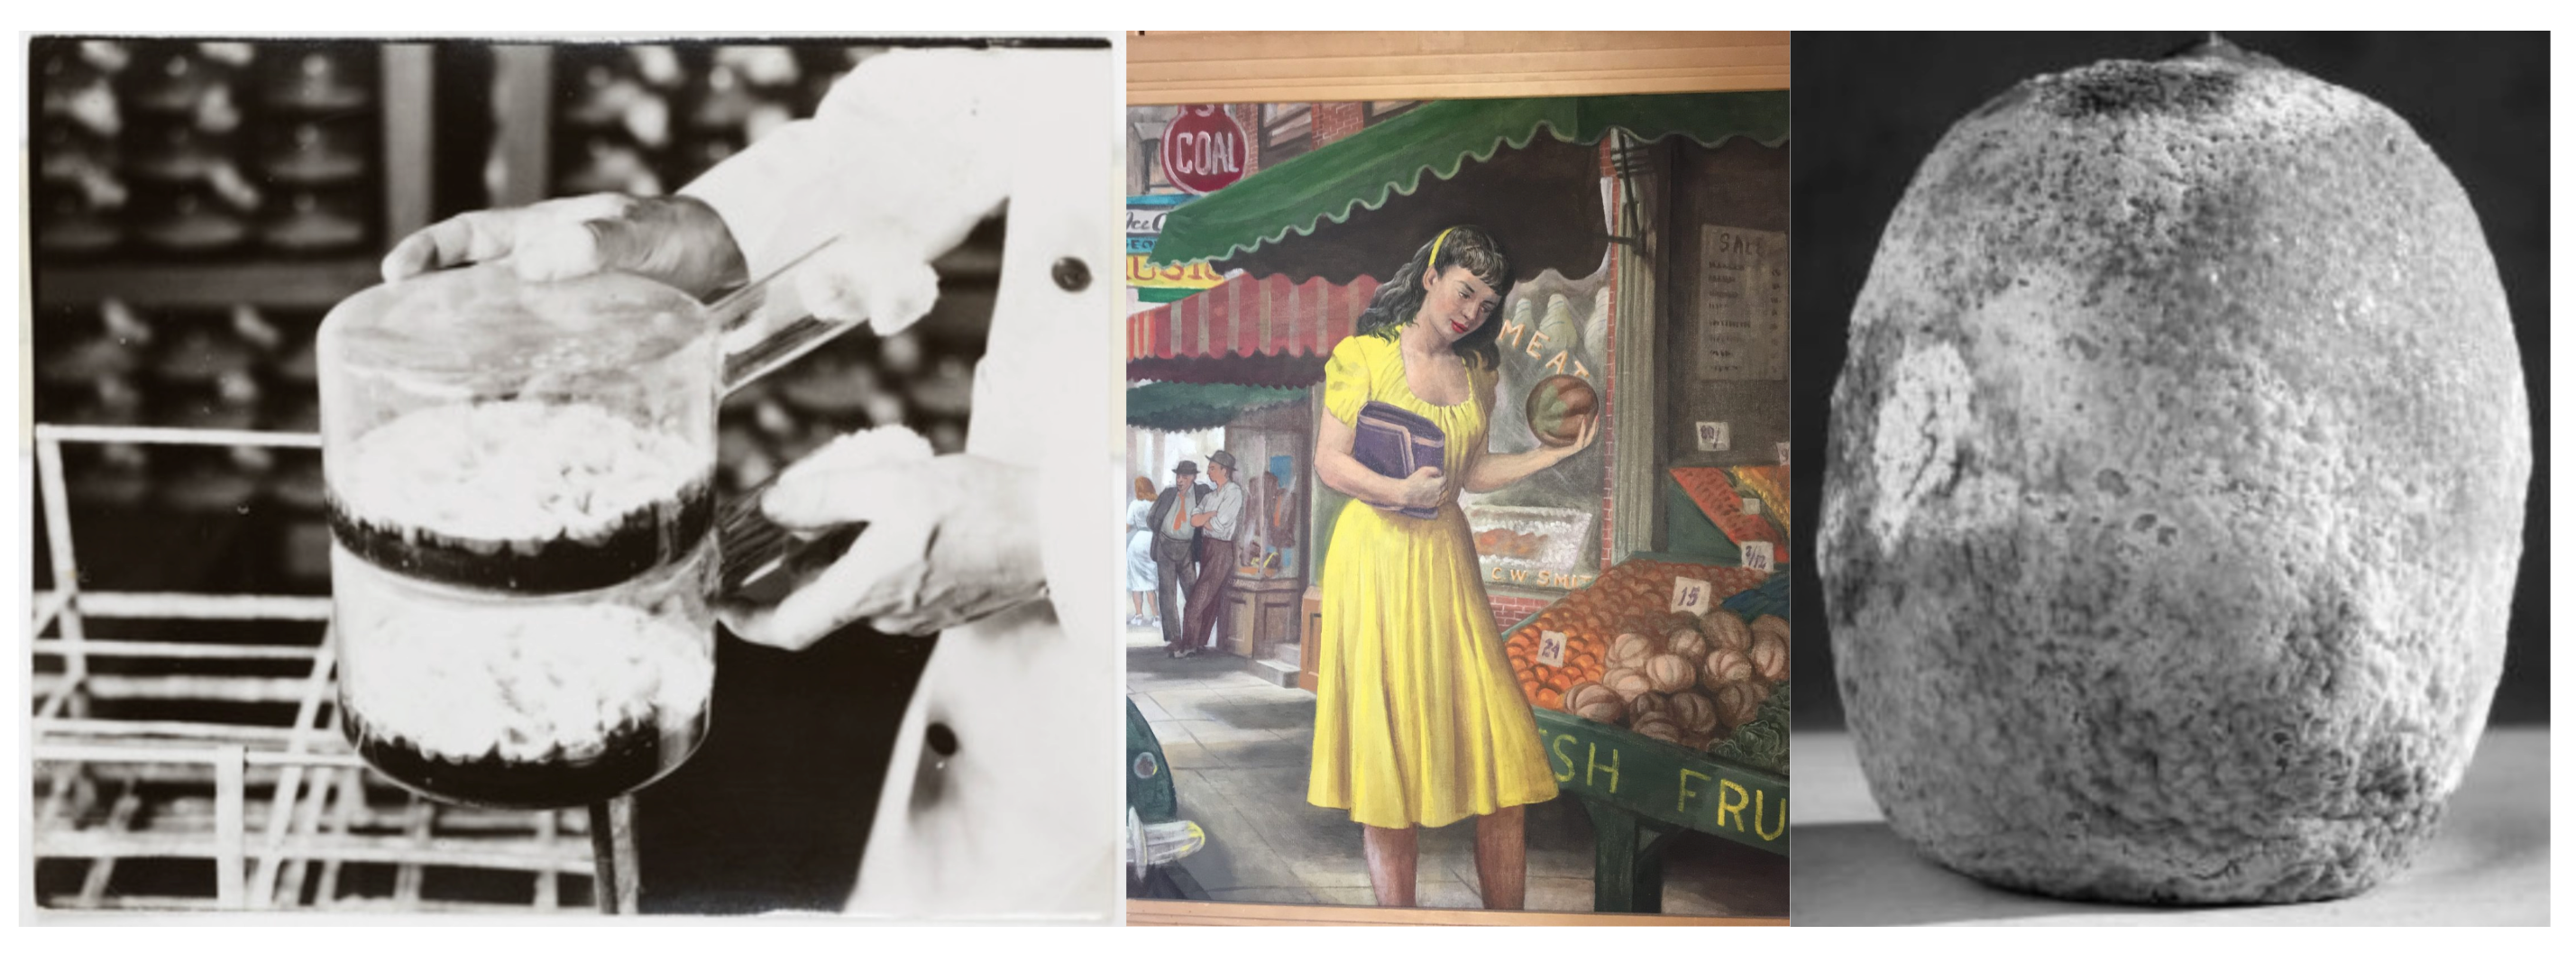
\includegraphics{images/moldymary.png}

}

\end{figure}

}

\caption{\label{fig-moldymarry}Penicillin fermentation (left panel),
Douglas Gorsline's 1948 painting of ``Moldy Mary'' in Peoria
Illinois(center panel), Purported original photograph of the moldy
mellon (right panel)}

\end{figure}

\begin{tcolorbox}[enhanced jigsaw, breakable, left=2mm, arc=.35mm, toprule=.15mm, colback=white, leftrule=.75mm, opacityback=0, rightrule=.15mm, bottomrule=.15mm]

For further reading about the history of penicillin development, see the
excellent book by Eric Lax: \emph{The Mold in Dr.~Florey's Coat}

\begin{figure}[H]

{\centering 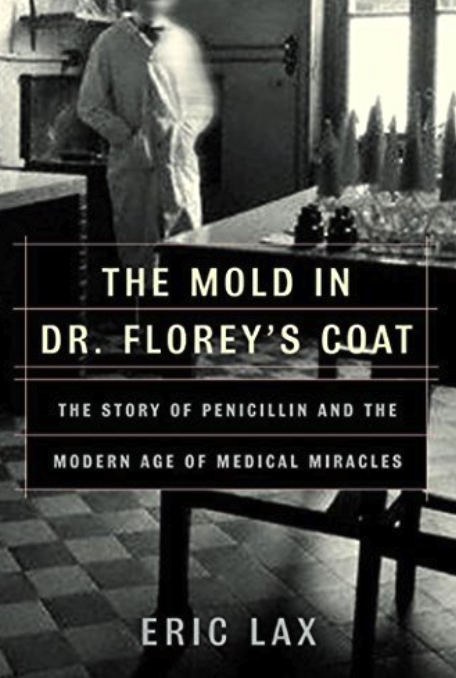
\includegraphics[width=1.5625in,height=\textheight]{images/lax.png}

}

\end{figure}

\end{tcolorbox}

In the early 1940s, Dorothy Hodgkin, a crystallography expert at Oxford
University, used X-rays to analyze the structure of various natural
products. In 1946, she determined the structure of penicillin, earning
her the Nobel Prize in Chemistry in 1964 (Figure~\ref{fig-hodgkin}).
Knowledge of the penicillin structure allowed scientists to modify
penicillin, leading to the development of semisynthetic versions.
Semisynthetic antimicrobials are chemically modified derivatives of
natural antibiotics, designed to broaden their bacterial targets,
increase stability, reduce toxicity, or confer other beneficial
properties for treating infections.

\begin{figure}

{\centering 

\begin{figure}

{\centering 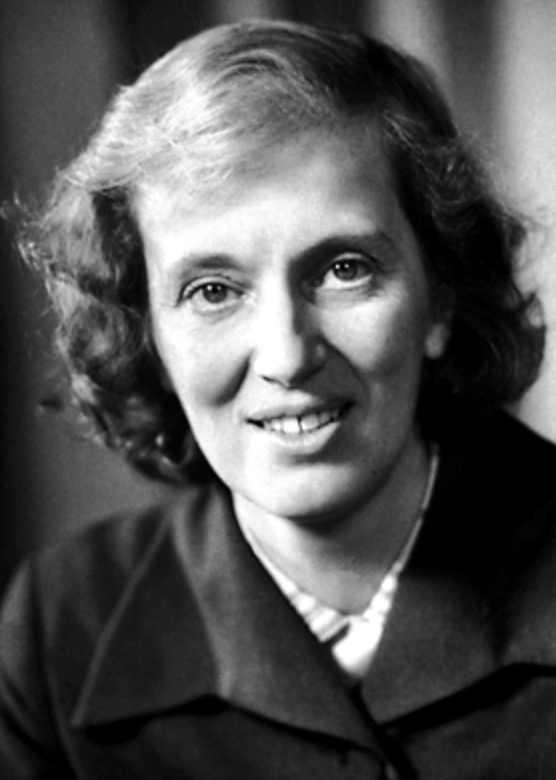
\includegraphics[width=1.5625in,height=\textheight]{images/hodgkin.png}

}

\end{figure}

}

\caption{\label{fig-hodgkin}Dorothy Hodgkin is the biochemist who solved
the xray crystal structure of penicillin opening the door for synthesis
of semisynthetic penicillins to combat resistance. Image source:
www.nobelprize.org}

\end{figure}

Penicillin is just one example of a natural antibiotic. In the 1940s,
Selman Waksman, a renowned soil microbiologist at Rutgers University,
and his research team discovered several antimicrobials, including
actinomycin, streptomycin, and neomycin. These findings stemmed from
Waksman's study of fungi and Actinobacteria, particularly soil bacteria
in the \emph{Streptomyces} genus known for their natural production of
diverse antimicrobials (Figure~\ref{fig-waksman}).

\begin{figure}

{\centering 

\begin{figure}

{\centering 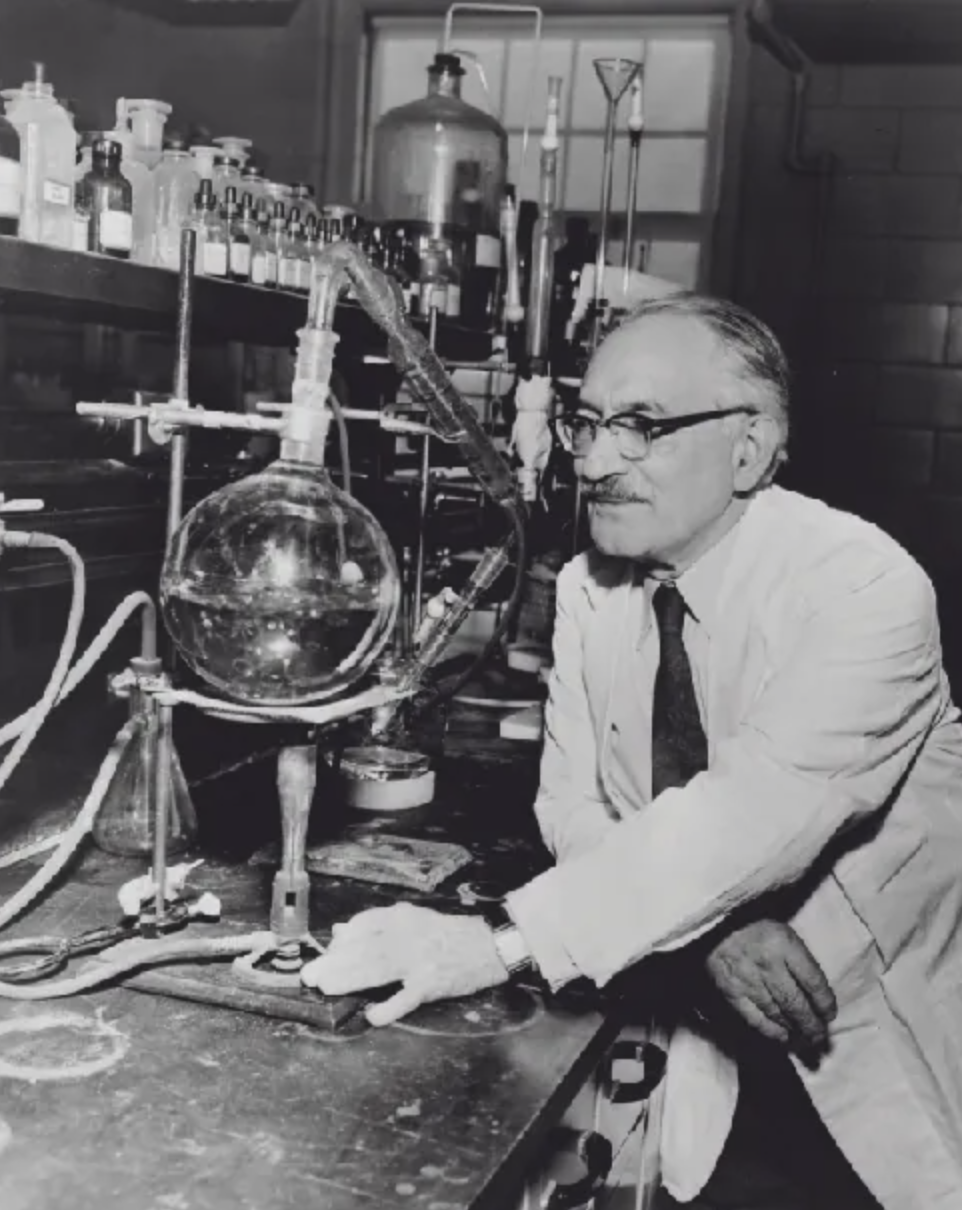
\includegraphics[width=3.125in,height=\textheight]{images/waksman.png}

}

\end{figure}

}

\caption{\label{fig-waksman}Selman Wakesman. Winner, Nobel Prize in
Medicine in 1952. Source: Rutgers University}

\end{figure}

Waksman's contributions earned him the Nobel Prize in Physiology and
Medicine in 1952. Actinomycetes, the source of more than half of all
natural antibiotics, continue to serve as a valuable resource for
discovering novel antimicrobial agents. Some researchers believe that we
have yet to fully explore the antimicrobial potential of this group.

The term \emph{antibiotic} was actually coined by Waksman.

\begin{figure}

{\centering 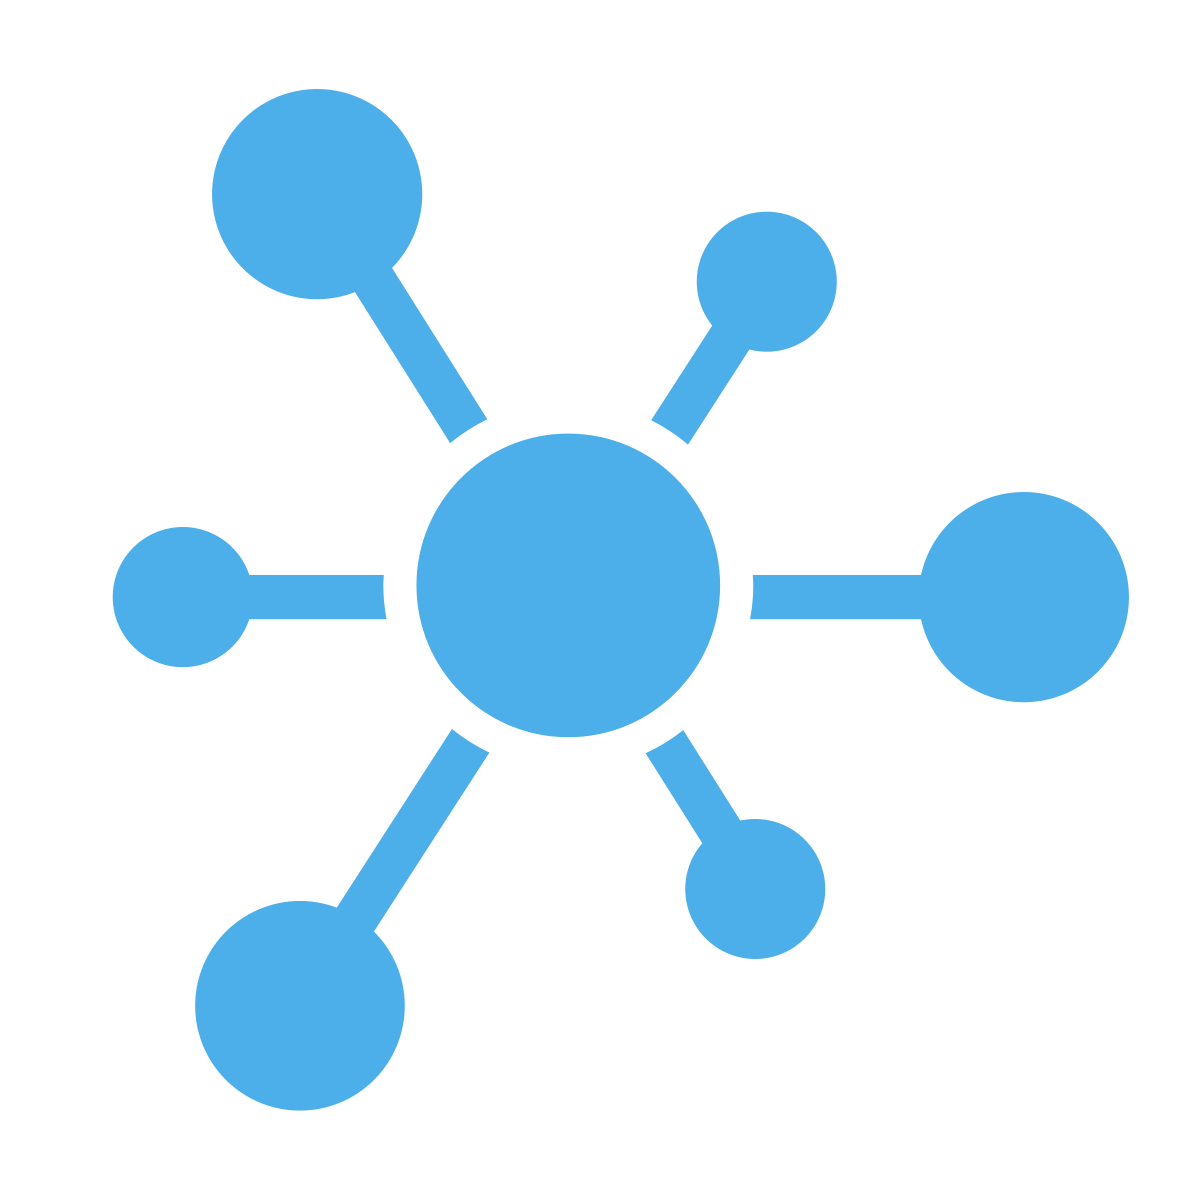
\includegraphics[width=1.04167in,height=\textheight]{images/breakblue.png}

}

\end{figure}

\hypertarget{history-of-antimicrobial-resistance}{%
\section{History of antimicrobial
resistance}\label{history-of-antimicrobial-resistance}}

Antimicrobial resistance is a natural occurrence as microbes adapt to
overcome antimicrobial compounds produced by other microorganisms.
However, the development and widespread use of antimicrobial drugs by
humans have added another selective pressure that drives further
evolution. Factors such as overuse, misuse, inappropriate use,
subtherapeutic dosing, and patient non-compliance and widespread use of
antibiotics in food production (livestock can accelerate the evolution
of drug resistance. Pathogens can develop resistance through chromosomal
mutations that are vertically transferred to subsequent generations or
through horizontal gene transfer facilitated by plasmids and
transposons, which can promote the spread of resistance.

Certain organisms, like \emph{Acinetobacter baumannii} or
\emph{Pseudomonas aeruginosa}, naturally possess the ability to develop
multiple types of resistance. On the other hand, organisms like
\emph{Klebsiella pneumoniae} have historically been treatable but are
now becoming highly resistant by acquiring new resistance elements.
There are also organisms, such as \emph{Streptococcus pyogenes}, that
have remained susceptible to ``old'' antibiotics like penicillin since
their introduction.

Antibiotic resistance in bacteria typically originates from specific
events. While resistance can arise within a bacterium through random
mutations affecting the target of the antibiotic or other essential
elements, it is more commonly acquired from other bacteria through the
transfer of mobile genetic elements. Bacteria have the ability to
exchange genes not only within their own species but also between
different species and even genera. The transfer of \textbf{plasmids},
circular DNA structures that can carry multiple genes including those
for antibiotic resistance, is a crucial mechanism for gene transmission
among bacteria. Plasmids are highly mobile and can encode for various
types of resistance that are unrelated, such as resistance to
cephalosporins through beta-lactamase production and resistance to
fluoroquinolones via efflux pumps. Through this gene swapping process, a
bacterium can become resistant to multiple antibiotics.

Penicillinase (enzymes produced by bacteria that destroy the beta-lactam
ring of penicillin) were already reported by 1940 prior to the first
clinical use of the drug.(Davies and Davies 2010) Alexander Fleming was
among the first physicians to caution about the risks of resistance to
penicillin if used too little or for a too short of period during
treatment.

\begin{tcolorbox}[enhanced jigsaw, breakable, left=2mm, arc=.35mm, toprule=.15mm, colback=white, leftrule=.75mm, opacityback=0, rightrule=.15mm, bottomrule=.15mm]

\begin{figure}[H]

{\centering 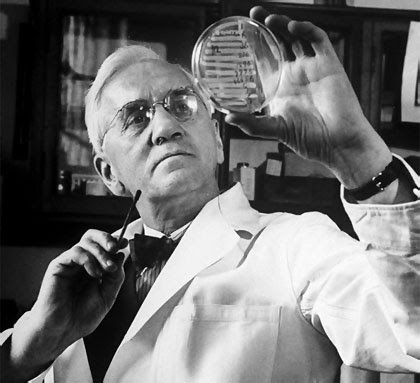
\includegraphics[width=1.5625in,height=\textheight]{images/alexflemming.jpeg}

}

\end{figure}

``It is not difficult to make microbes resistant to penicillin in the
laboratory by exposing them to concentrations not sufficient to kill
them, and the same thing has occasionally happened in the body. The time
may come when penicillin can be bought by anyone in the shops. Then
there is the danger that the ignorant man may easily under-dose himself
and by exposing his microbes to non-lethal quantities of the drug make
them resistant.'' Sir Alexander Fleming, Nobel Prize Lecture, December
11, 1944

\end{tcolorbox}

\begin{figure}

{\centering 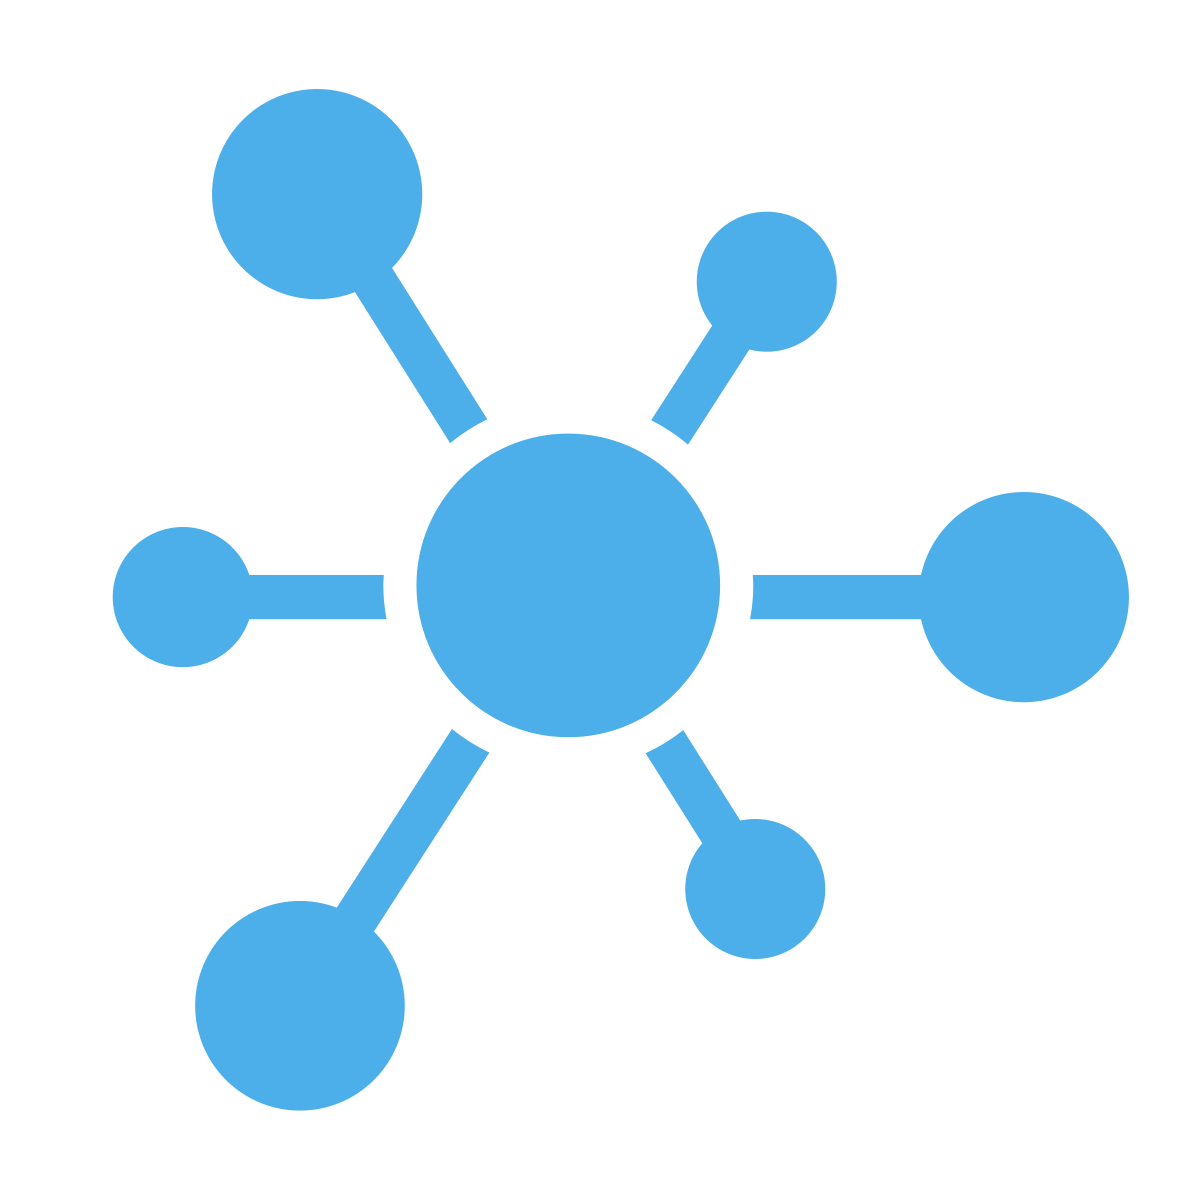
\includegraphics[width=1.04167in,height=\textheight]{images/breakblue.png}

}

\end{figure}

\hypertarget{mechanisms-of-antimicrobial-drugs}{%
\section{Mechanisms of antimicrobial
drugs}\label{mechanisms-of-antimicrobial-drugs}}

Selective toxicity is a crucial trait for antimicrobial drugs, as it
means they can specifically target and harm microbial organisms while
causing minimal harm to the host. Antibacterial drugs are the most
commonly used antimicrobials because they have a wider range of unique
targets in prokaryotic cells compared to fungi, parasites, and viruses.
Each class of antibacterial drugs has its own distinct mode of action,
which describes how the drug affects microbes at the cellular level. See
Figure~\ref{fig-bactmechanism} and Table~\ref{tbl-mechanism}).

\begin{figure}

{\centering 

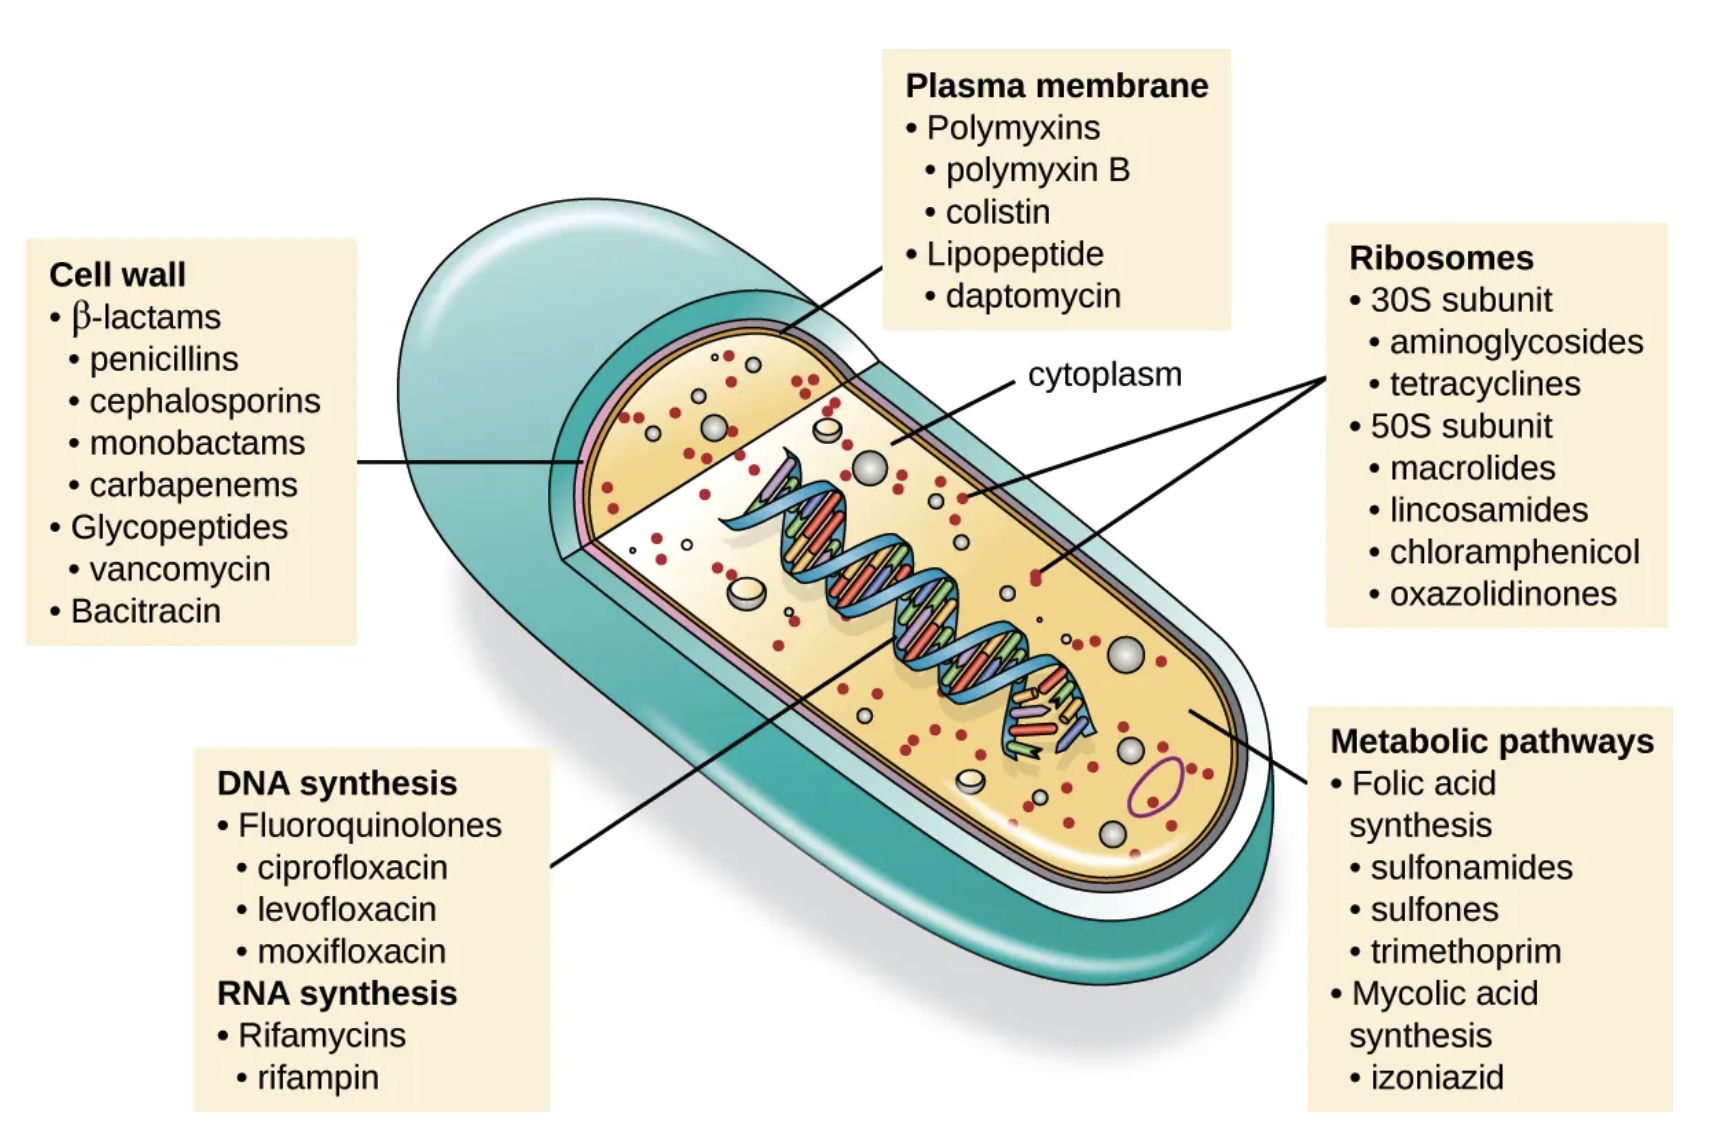
\includegraphics{images/bactmechanism.png}

}

\caption{\label{fig-bactmechanism}Mechanisms of antibacterial agents.
Image source: OpenStax-Rice University.}

\end{figure}

\hypertarget{tbl-mechanism}{}
\begin{longtable}[]{@{}
  >{\raggedright\arraybackslash}p{(\columnwidth - 4\tabcolsep) * \real{0.3333}}
  >{\raggedright\arraybackslash}p{(\columnwidth - 4\tabcolsep) * \real{0.3125}}
  >{\raggedright\arraybackslash}p{(\columnwidth - 4\tabcolsep) * \real{0.3490}}@{}}
\caption{\label{tbl-mechanism}Mechanism of antimicrobial
agents}\tabularnewline
\toprule\noalign{}
\begin{minipage}[b]{\linewidth}\raggedright
\textbf{Common Antibacterial Drugs by Mode of Action}
\end{minipage} & \begin{minipage}[b]{\linewidth}\raggedright
\end{minipage} & \begin{minipage}[b]{\linewidth}\raggedright
\end{minipage} \\
\midrule\noalign{}
\endfirsthead
\toprule\noalign{}
\begin{minipage}[b]{\linewidth}\raggedright
\textbf{Common Antibacterial Drugs by Mode of Action}
\end{minipage} & \begin{minipage}[b]{\linewidth}\raggedright
\end{minipage} & \begin{minipage}[b]{\linewidth}\raggedright
\end{minipage} \\
\midrule\noalign{}
\endhead
\bottomrule\noalign{}
\endlastfoot
Mode of Action & Target & Drug Class \\
Inhibit cell wall biosynthesis & Penicillin-binding proteins &
β-lactams: penicillins, cephalosporins, monobactams, carbapenems \\
Peptidoglycan subunits & Glycopeptides & \\
Peptidoglycan subunit transport & Bacitracin & \\
Inhibit biosynthesis of proteins & 30S ribosomal subunit &
Aminoglycosides, tetracyclines \\
50S ribosomal subunit & Macrolides, lincosamides, chloramphenicol,
oxazolidinones & \\
Disrupt membranes & Lipopolysaccharide, inner and outer membranes &
Polymyxin B, colistin, daptomycin \\
Inhibit nucleic acid synthesis & RNA & Rifamycin \\
DNA & Fluoroquinolones & \\
Antimetabolites & Folic acid synthesis enzyme & Sulfonamides,
trimethoprim \\
Mycolic acid synthesis enzyme & Isonicotinic acid hydrazide & \\
Mycobacterial adenosine triphosphate (ATP) synthase inhibitor &
Mycobacterial ATP synthase & Diarylquinoline \\
\end{longtable}

\begin{figure}

{\centering 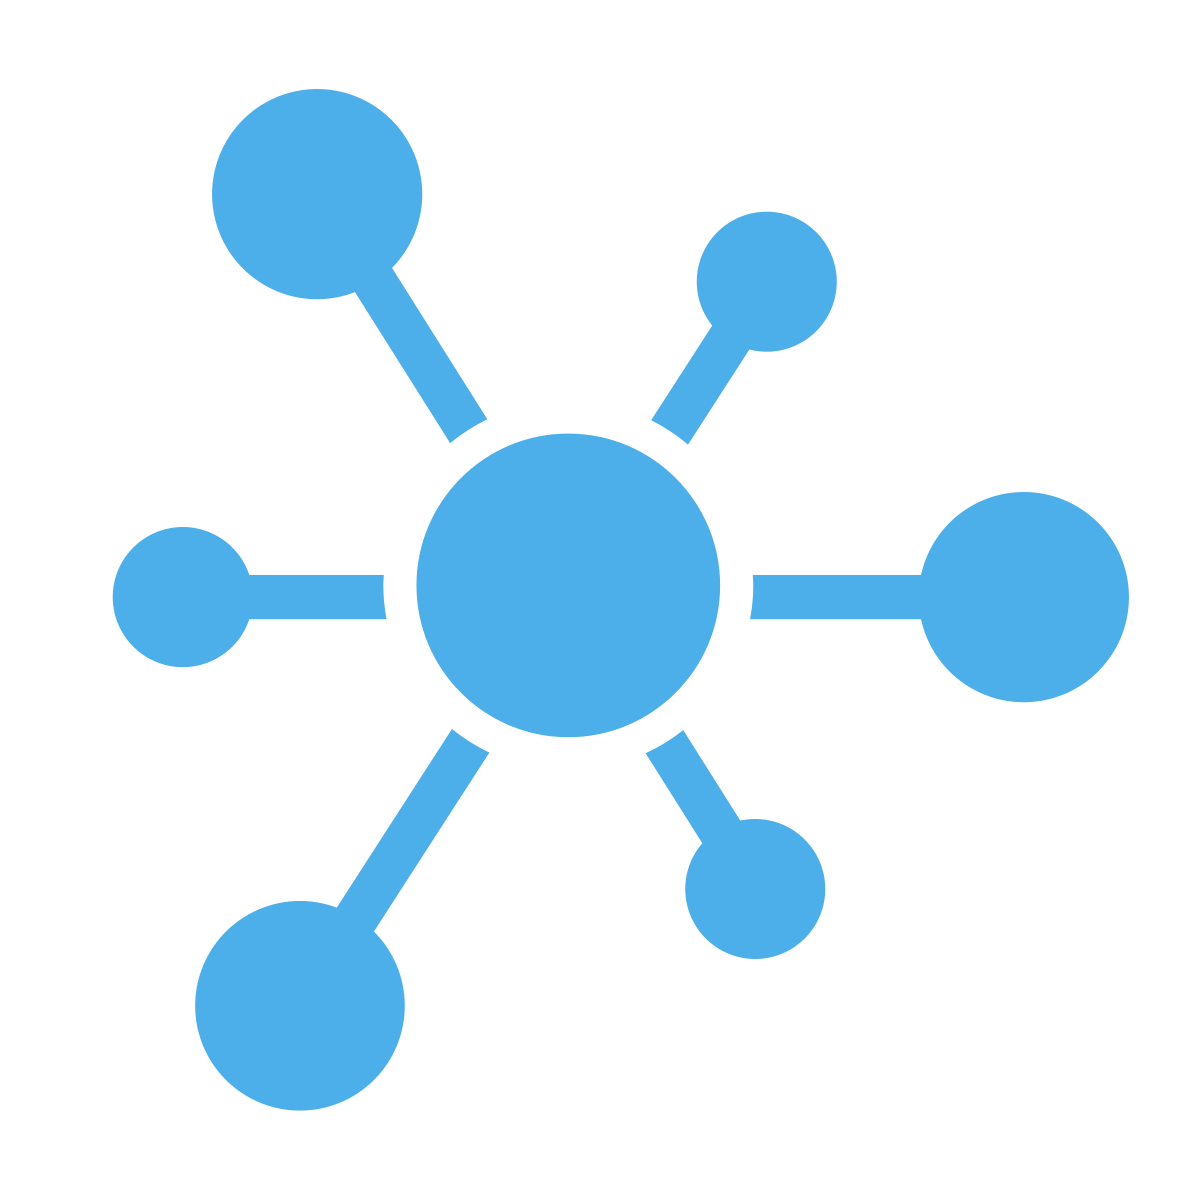
\includegraphics[width=1.04167in,height=\textheight]{images/breakblue.png}

}

\end{figure}

\hypertarget{mechanisms-of-antibiotic-resistance}{%
\section{Mechanisms of antibiotic
resistance}\label{mechanisms-of-antibiotic-resistance}}

There are several common mechanisms for drug resistance, which are
summarized in Figure~\ref{fig-resistance}. These mechanisms include
enzymatic modification of the drug, modification of the antimicrobial
target, and prevention of drug penetration or accumulation.

\begin{figure}

{\centering 

\begin{figure}

{\centering 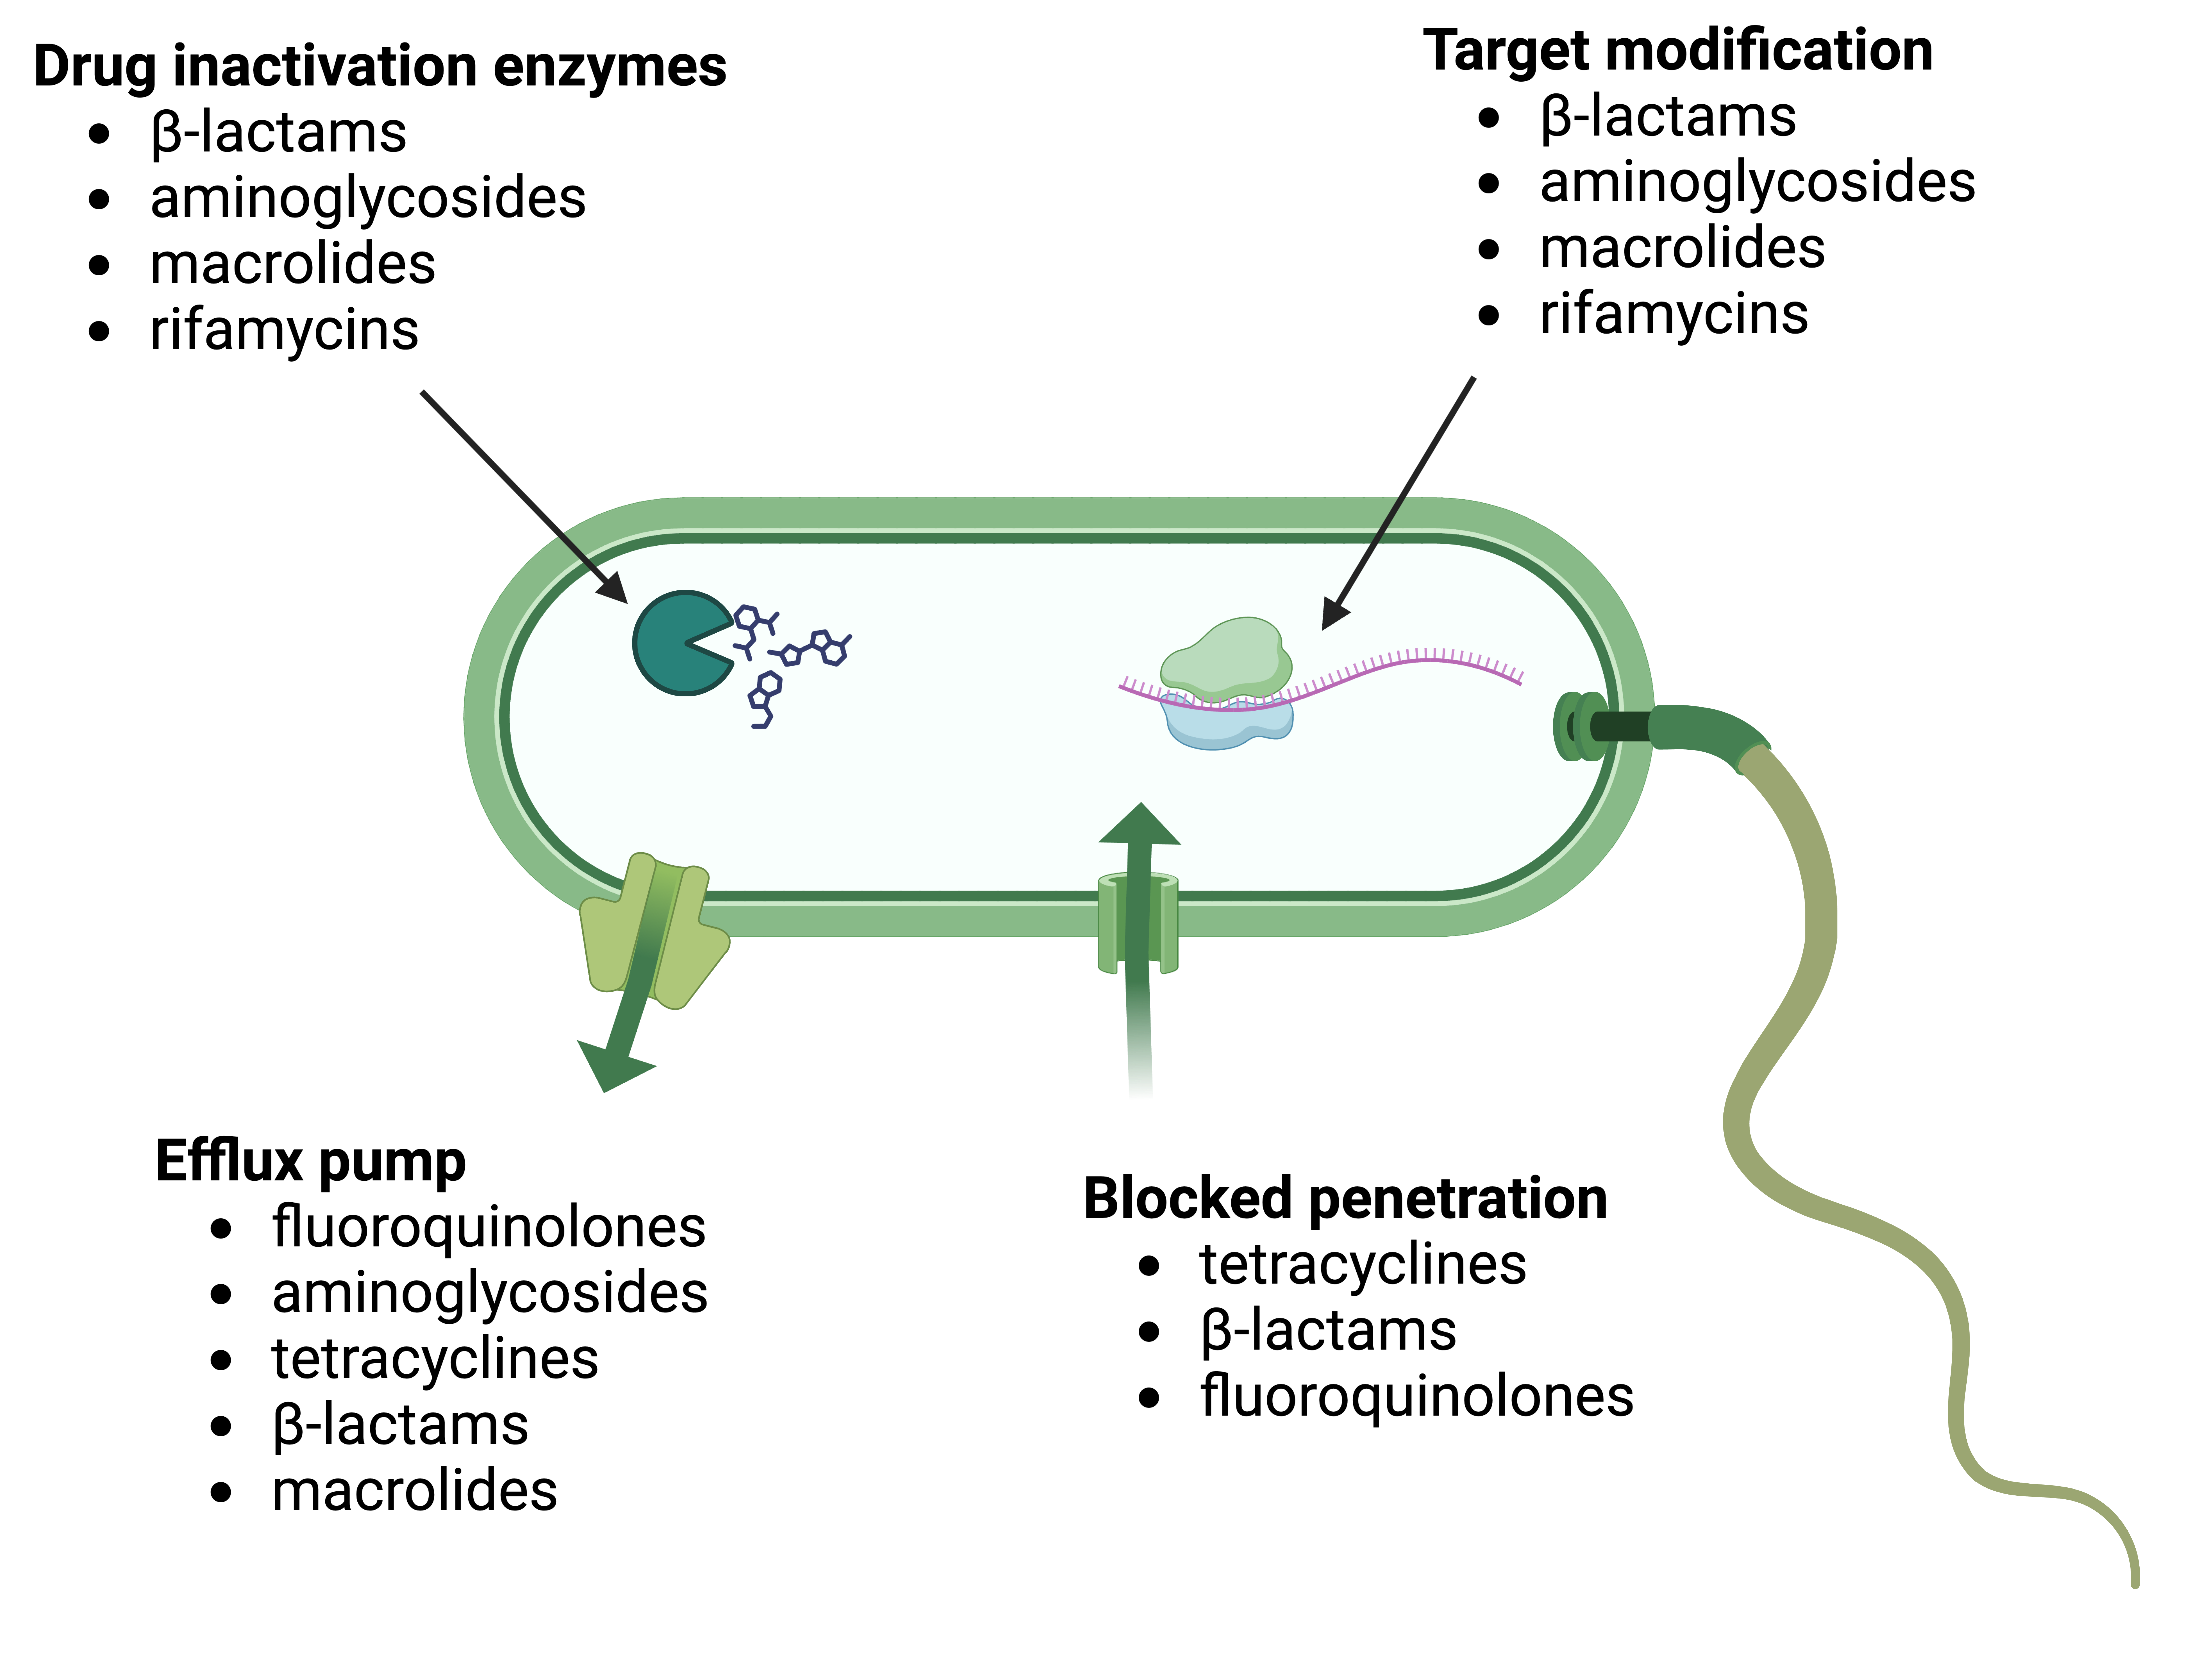
\includegraphics{images/resistance.png}

}

\end{figure}

}

\caption{\label{fig-resistance}Overview of antimicrobial resistance
mechanisms}

\end{figure}

\textbf{Drug Modification or Inactivation:} Resistance genes can produce
enzymes that modify or hydrolyse antimicrobials, rendering them
inactive. This mechanism is common in various antimicrobials, such as
aminoglycosides and β-lactams. Aminoglycoside resistance can occur
through the transfer of chemical groups to the drug molecule,
interfering with its binding. β-lactam resistance involves the enzymatic
hydrolysis of the β-lactam bond in the drug molecule's β-lactam ring,
leading to loss of antibacterial activity. Rifampin can be inactivated
through glycosylation, phosphorylation, or ADP ribosylation, while
macrolides and lincosamides can be enzymatically inactivated or
modified.

\textbf{Prevention of Cellular Uptake or Efflux:} Some microbes develop
resistance by hindering the accumulation of antimicrobial drugs,
preventing them from reaching their targets. Gram-negative pathogens can
alter outer membrane lipid composition, porin channel selectivity, or
porin channel concentrations. For instance, \emph{Pseudomonas
aeruginosa} reduces the amount of its OprD porin to resist carbapenems.
Efflux pumps are produced by many gram-positive and gram-negative
bacteria to actively transport drugs out of the cell, preventing
effective drug accumulation. Efflux pumps can confer resistance to
β-lactams, tetracyclines, and fluoroquinolones.

\textbf{Target Modification:} Structural changes in antimicrobial drug
targets can prevent drug binding, leading to resistance. Spontaneous
mutations in genes encoding antibacterial drug targets allow bacteria to
develop resistance. For example, changes in penicillin-binding proteins
(PBPs) can inhibit the binding of β-lactam drugs, providing resistance.
Streptococcus pneumoniae alters its own PBPs, while \emph{Staphylococcus
aureus} acquires low-affinity PBPs to resist methicillin. Other examples
include alterations in ribosome subunits, lipopolysaccharide structure,
RNA polymerase, DNA gyrase, metabolic enzymes, and peptidoglycan subunit
peptide chains.

\textbf{Target Overproduction or Enzymatic Bypass:} In antimetabolite
drugs that target specific enzymes, resistance can occur through target
overproduction or the development of bypass mechanisms. Microbes may
produce excess target enzymes, ensuring enough enzyme activity despite
the presence of the drug. Alternatively, they may develop bypass
pathways that do not rely on the functional target enzyme. Sulfonamide
resistance can occur through these mechanisms. Vancomycin resistance in
\emph{S. aureus} involves decreased cross-linkage of peptide chains in
the cell wall, providing more targets for vancomycin binding.

\textbf{Target Mimicry:}A recently discovered resistance mechanism
called target mimicry involves the production of proteins that prevent
drugs from binding to their targets. For example, \emph{Mycobacterium
tuberculosis} can develop fluoroquinolone resistance by producing a
protein called MfpA, which resembles DNA. MfpA binds to DNA gyrase,
preventing fluoroquinolones from binding.

\begin{figure}

{\centering 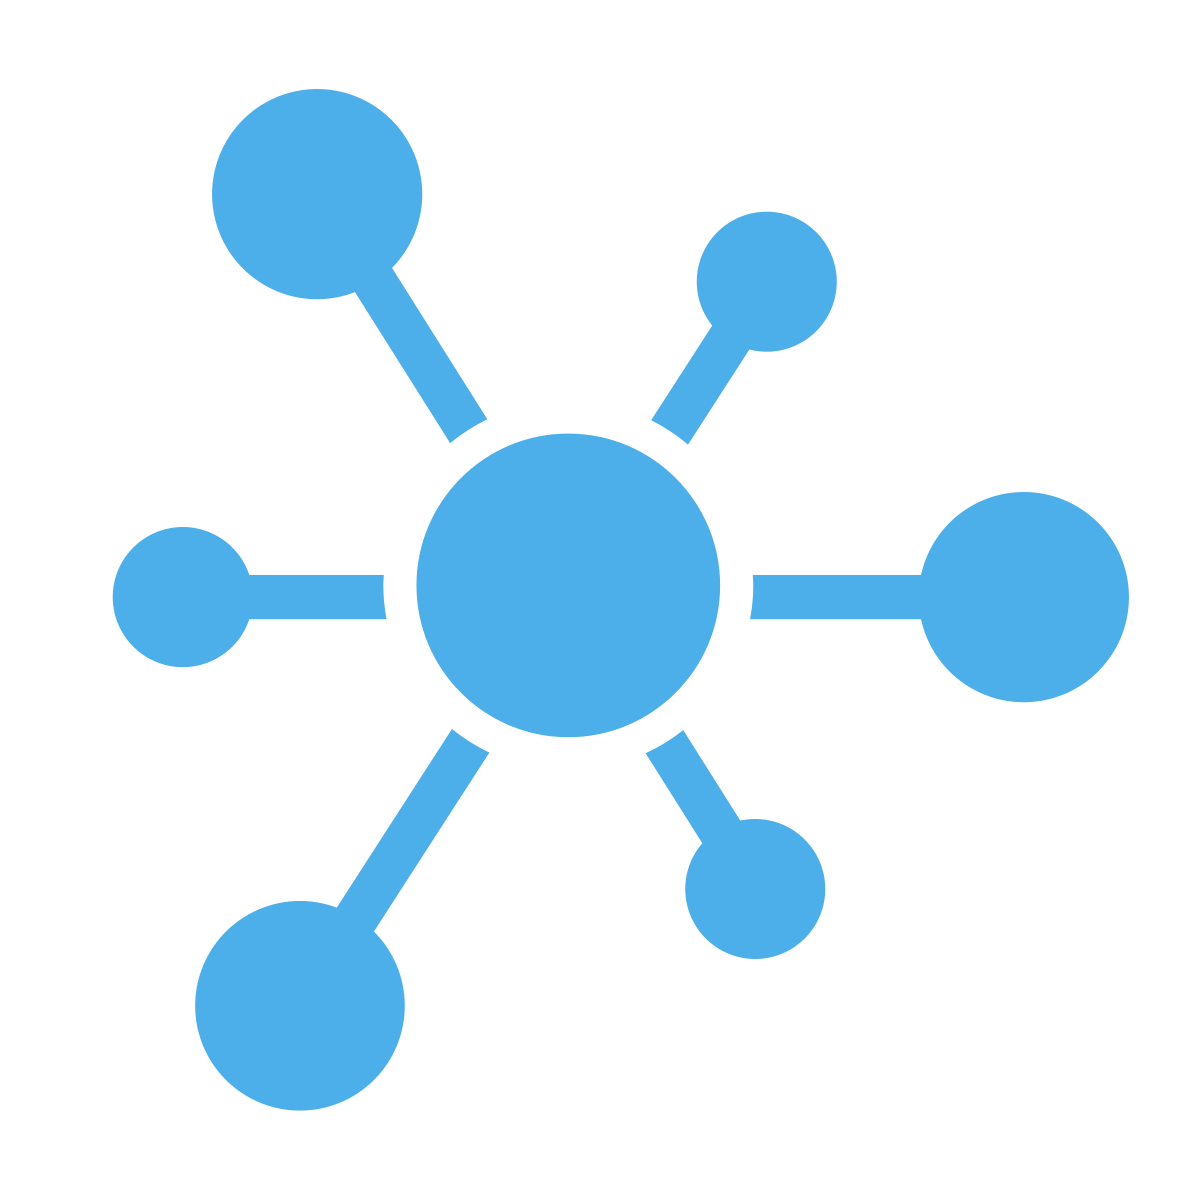
\includegraphics[width=1.04167in,height=\textheight]{images/breakblue.png}

}

\end{figure}

\hypertarget{antibiotic-discovery-to-the-rescue}{%
\section{Antibiotic discovery to the
rescue}\label{antibiotic-discovery-to-the-rescue}}

Initially, antibiotic discovery seemed to keep pace with emerging
resistance as a host of new chemical classes were developed and
introduced in the 1950s-1980's. For the first half of the century, the
repeated and successful response to emerging resistance was to discover
a new class of antibiotics.

Yet by the 1980's, the discovery of new agents began to slow and this
strategy began to fail Figure~\ref{fig-abxtimeline}. The last truly
``new'' antibiotic class discovered that reached the market was in 1987.
Since then, there has been a lack of innovation in the field, and today
there are few novel antibiotic classes in the drug pipeline.

\begin{figure}

{\centering 

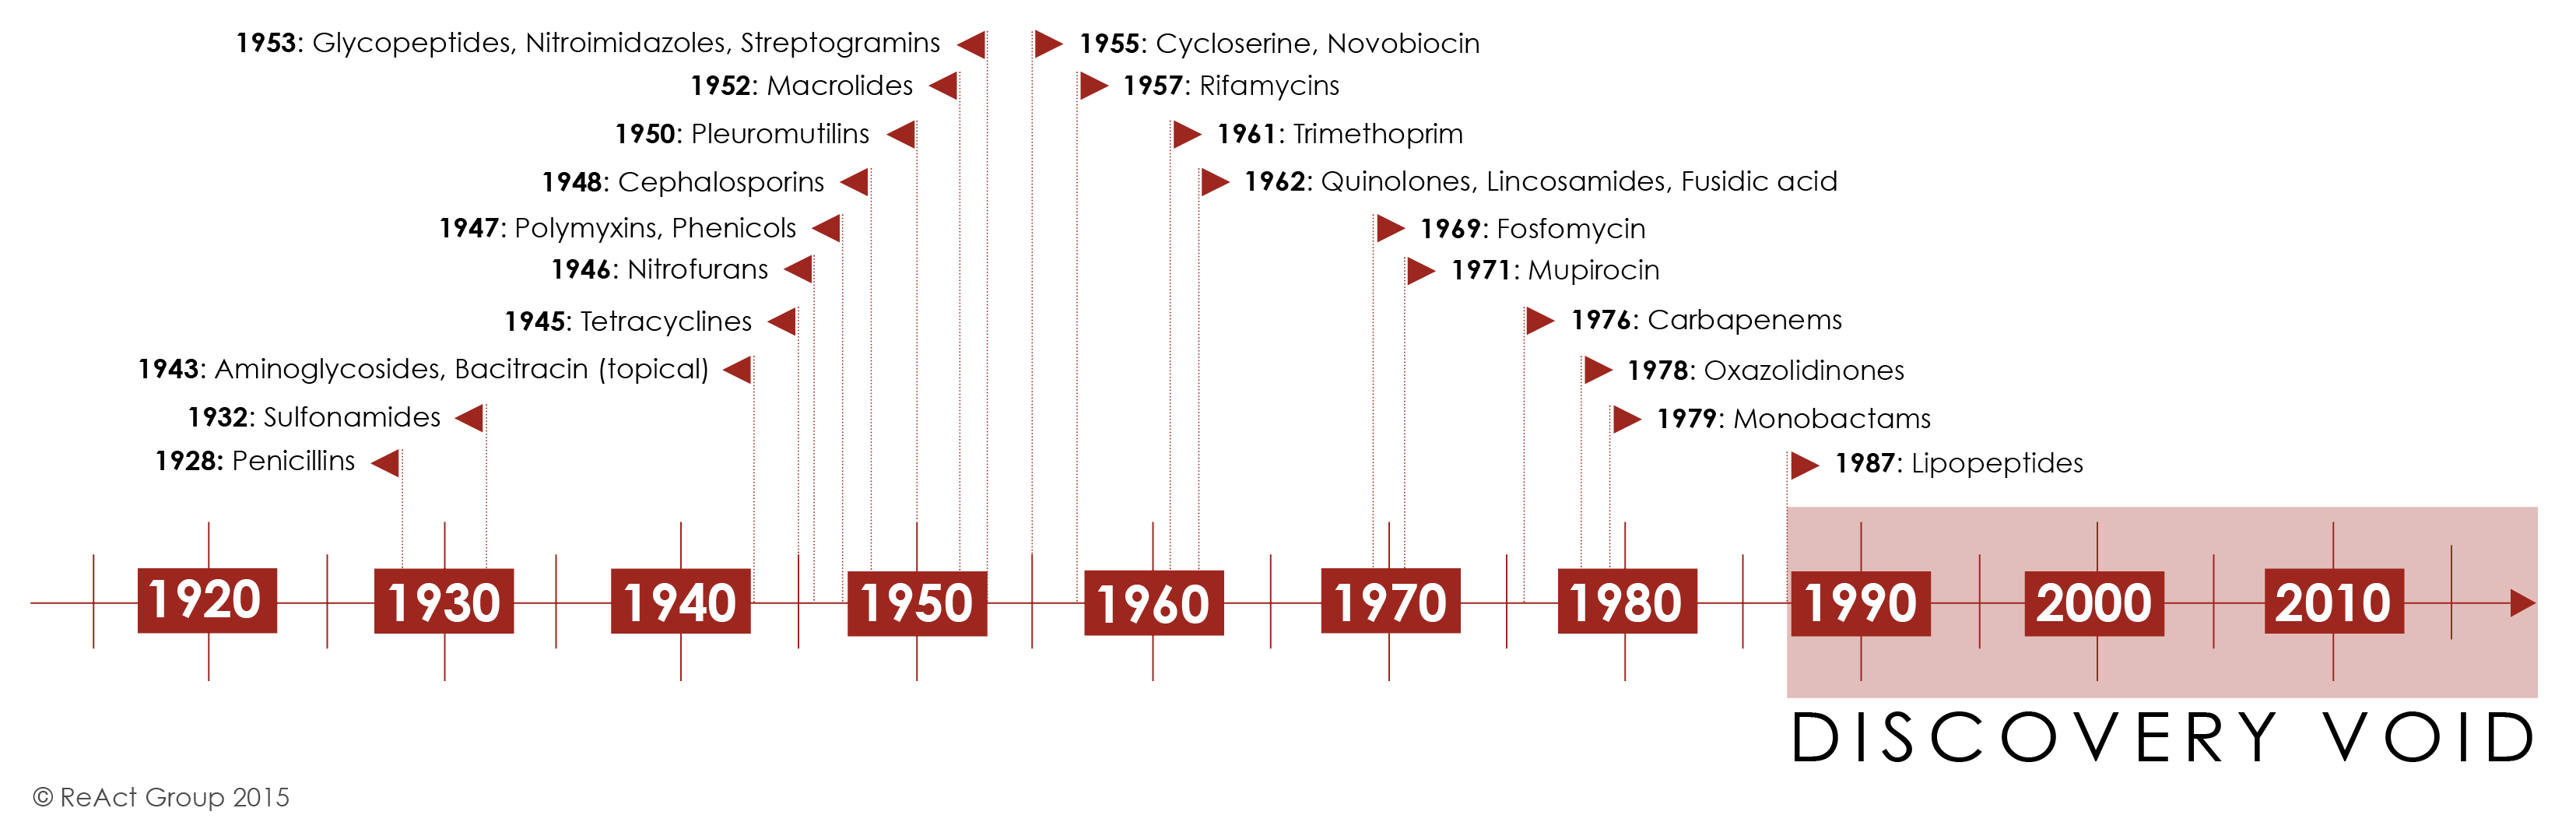
\includegraphics{images/ab-discovery-timeline.png}

}

\caption{\label{fig-abxtimeline}Antibiotic discovery timeline. Source:
www.reactgroup.org}

\end{figure}

The slowdown in new antibiotic development is occurring at a time when
resistance, particularly to penicillins and beta-lactam antibiotics is
dramatically increasing due to the wide spread and adaptation of enzymes
that hydrolyze this drug class-beta lactamases
(Figure~\ref{fig-betalactmases}).

\begin{figure}

{\centering 

\begin{figure}

{\centering 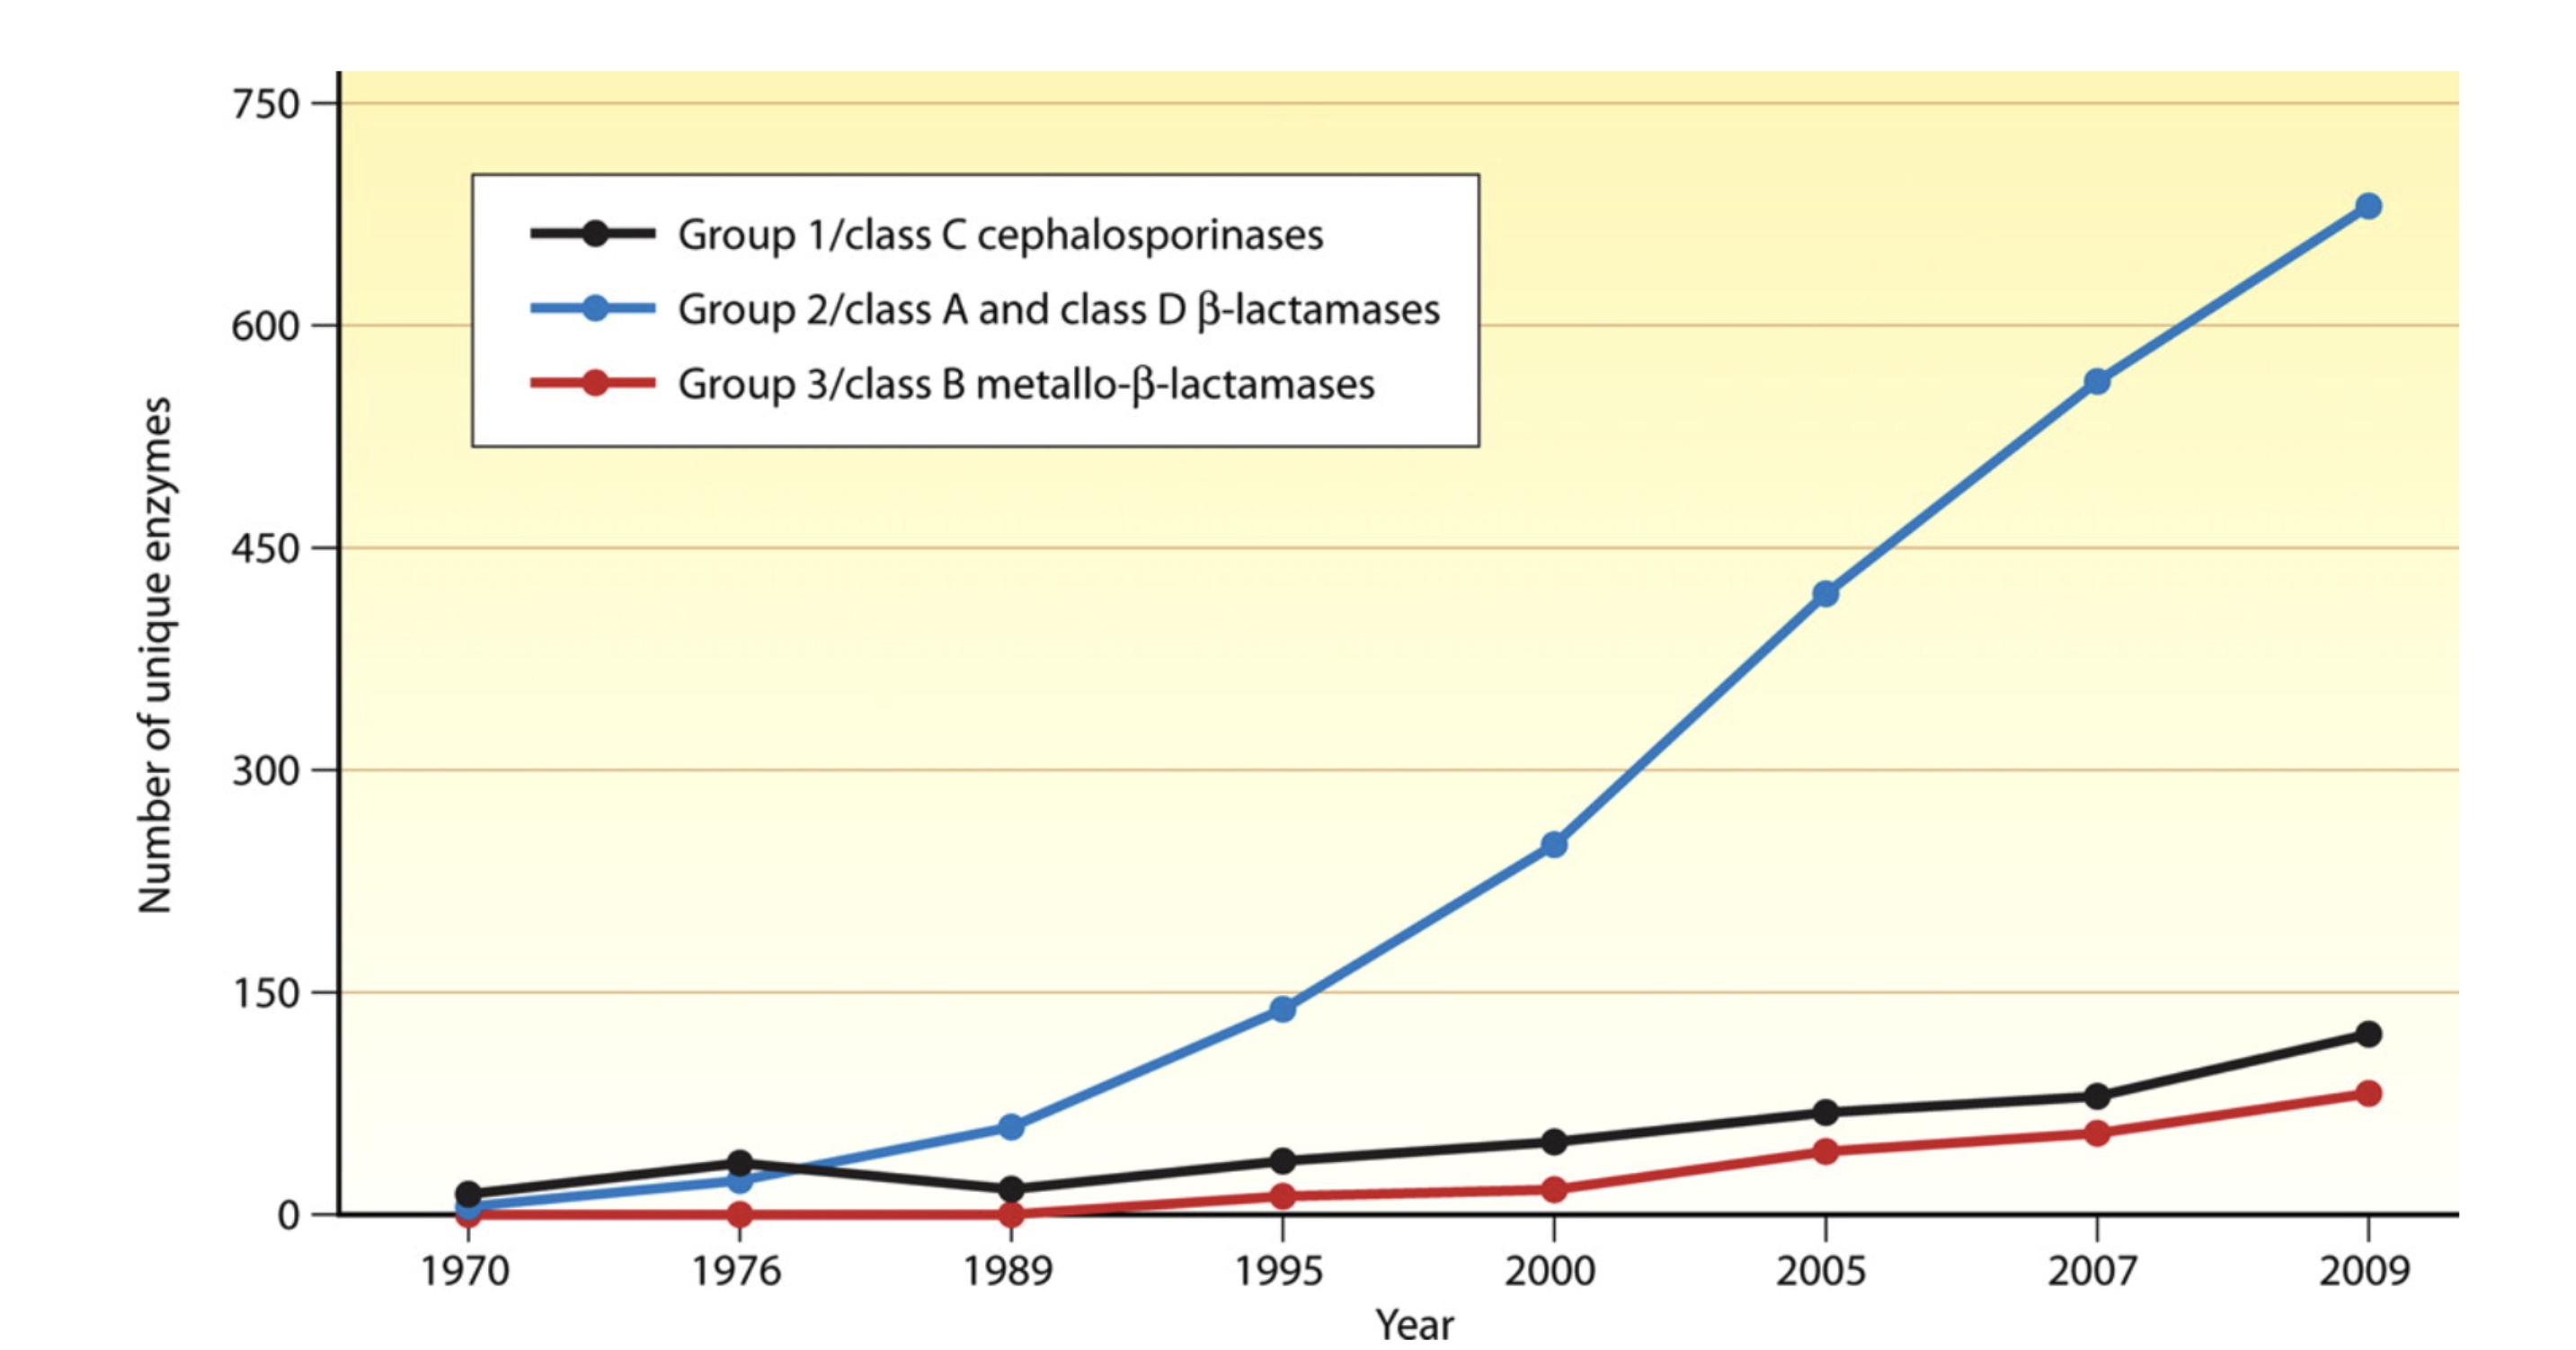
\includegraphics[width=15.625in,height=\textheight]{images/betalactamases.png}

}

\end{figure}

}

\caption{\label{fig-betalactmases}Marked increased in beta-lactamases
over the last 4 decades. Figure is form Bush et al. (Bush and Jacoby
2010)}

\end{figure}

Antibiotic use in humans in only one of many drivers of antimicrobial
resistance, as increasing use of antimicrobials in livestock for growth
promotion, of agriculture to prevent spoilage, or release of
antimicrobials into the environmental waste-water contributes to the
\emph{resistome} - the total burden of antibiotic resistance genes in
the environment (Figure~\ref{fig-resistancedrivers}\}. Therefore,
strategies to combat antimicrobial resistance have taken on a
\textbf{One Health Approach- i.e.~interdisciplinary and collaborative
strategies that considers the interconnectedness of human health, animal
health, and the environment. This approach promotes cooperation between
various sectors, such as human medicine, veterinary medicine,
environmental science, and public health, to achieve optimal health
outcomes for all.}

\begin{figure}

{\centering 

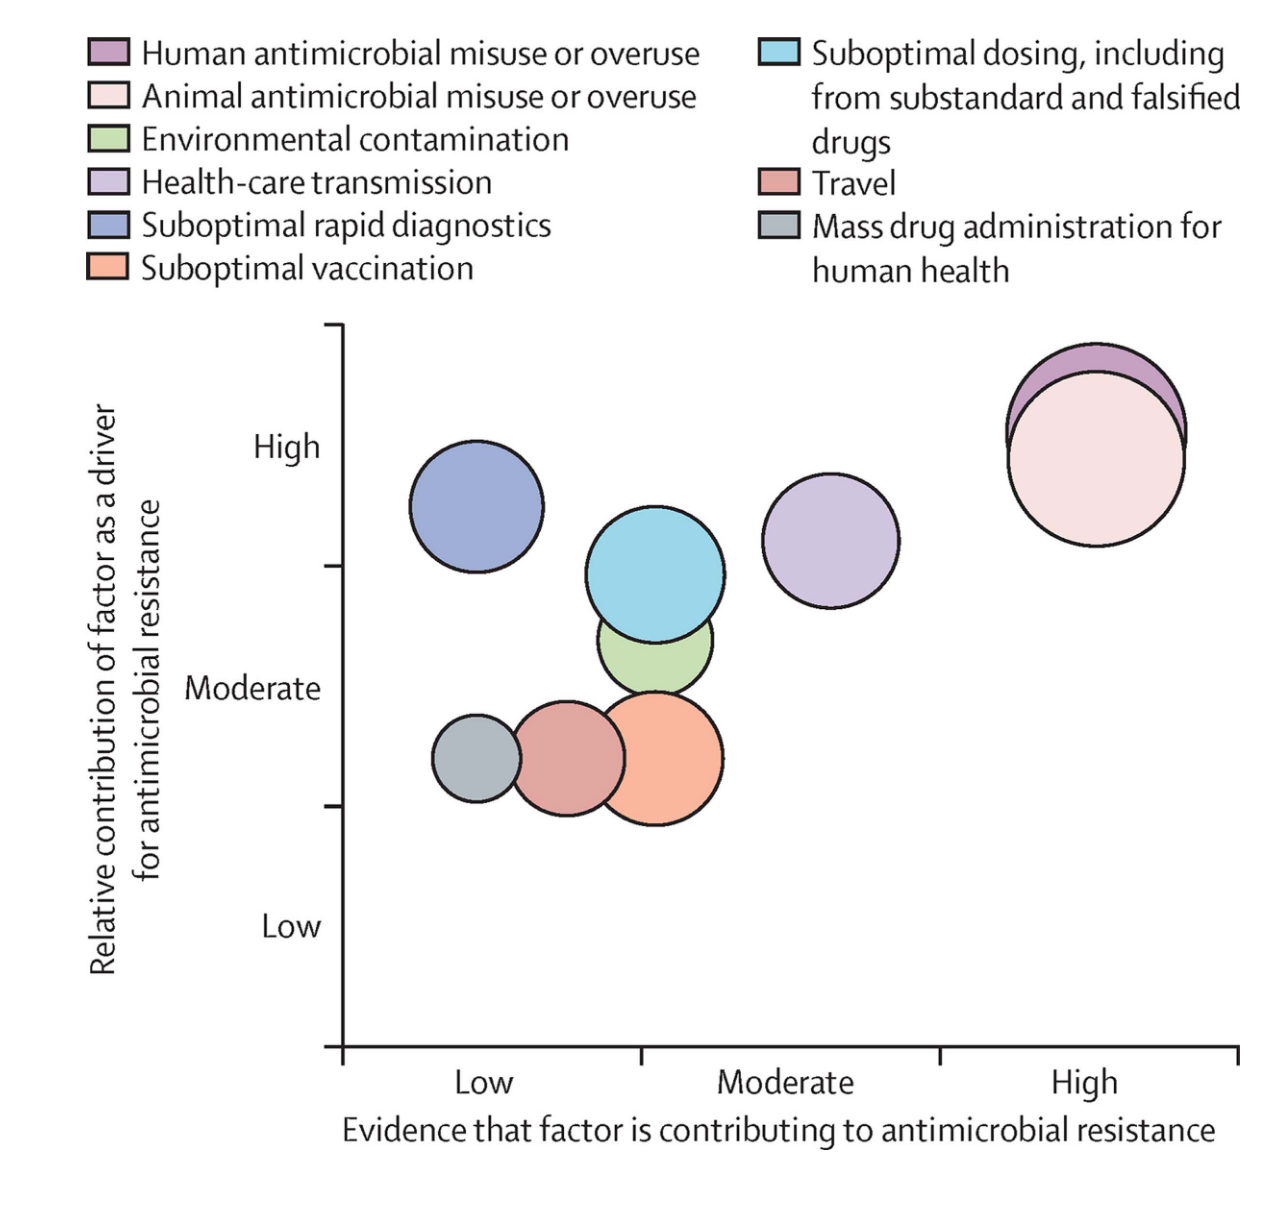
\includegraphics[width=5.20833in,height=\textheight]{images/modifiablerisk.png}

}

\caption{\label{fig-resistancedrivers}Modifiable risk factors that drive
antimicrobial resistance. Figure form Homes et al.(Holmes et al. 2016)}

\end{figure}

\textbf{The consequences of faltering antibiotic discovery are now being
felt worldwide as more and more bacterial infections are becoming harder
to treat.} Especially worrisome is the lack of antibiotics against
common Gram-negative bacteria (i.e.~\emph{Escherichia coli, Klebsiella
pneumonia, Pseudomonas aeruginosa, Acinetobacter baumannii}) that are
increasingly resistant to all but last-line antibiotics. The rapid
global spread of multi- and pan-resistant bacteria, also known in the
lay press as ``superbugs,'' can cause infections that are not treatable
with existing antibiotics.

\begin{tcolorbox}[enhanced jigsaw, toptitle=1mm, colframe=quarto-callout-note-color-frame, arc=.35mm, rightrule=.15mm, title=\textcolor{quarto-callout-note-color}{\faInfo}\hspace{0.5em}{How quickly can antibiotics develop resistance?}, leftrule=.75mm, opacityback=0, opacitybacktitle=0.6, breakable, coltitle=black, toprule=.15mm, colback=white, colbacktitle=quarto-callout-note-color!10!white, bottomtitle=1mm, titlerule=0mm, bottomrule=.15mm, left=2mm]

Click this link to watch a YOUTUBE video of how quickly
\emph{Escherichia coli} and
\href{https://www.youtube.com/watch?v=bDa4-nSc7J8}{develop resistance to
ciprofloxacin.}

Another excellent YOUTUBE video on the crises of antibiotic resistance
and the dwindleing antibiotic pipeline was presented by the FRONTLINE
Program on the :
\href{https://www.youtube.com/watch?v=EkyAuG9RSSU\&t=1250s}{When
Antibiotics Don't Work}

\end{tcolorbox}

\hypertarget{global-response-to-antimicrobial-resistance}{%
\section*{Global response to antimicrobial
resistance}\label{global-response-to-antimicrobial-resistance}}
\addcontentsline{toc}{section}{Global response to antimicrobial
resistance}

\markright{Global response to antimicrobial resistance}

Recognizing the growing global threat of antibiotic resistance (AMR) on
human health but also the economy and human development, The World
Health Organization (WHO) and The Organisation for Animal Health (OIE)
developed in 2001 a Global Plan for Containment of Antimicrobial
Resistance that subsequently led to a
\href{https://www.who.int/publications/i/item/9789241509763}{Global
Action Plan for AMR} in 2017 and more recently a
\href{https://www.who.int/news/item/30-07-2021-call-to-action-on-antimicrobial-resistance-2021}{``Call
to Action on Antimicrobial Resistance''} in 2021. The plan outlines 21
strategies and 5 strategic objectives action plans that should be
implemented in member states to address AMR. These include:

\begin{enumerate}
\def\labelenumi{\arabic{enumi}.}
\tightlist
\item
  Improvements in the awareness and understanding of antimicrobial
  resistance through effective communication, education and training
\item
  Strengthening of knowledge and evidence base of AMR through
  surveillance and research
\item
  Reductions in the incidence of infection through effective sanitation,
  hygiene and infection prevention measures
\item
  Optimization the use of antimicrobial medicines in human and animal
  health
\item
  Development of an economic case for sustainable investment in AMR
  research that takes account of the needs of all countries, and
  increase investment in new medicines, diagnostic tools, vaccines and
  other interventions
\end{enumerate}

One aspect of this action plan was the development of Global
Antimicrobial Resistance and Use Surveillance System (GLASS). A link the
2022 report can be \href{glass2022.pdf}{here}

The WHO also proposed a
\href{https://www.who.int/medicines/publications/WHO-PPL-Short_Summary_25Feb-ET_NM_WHO.pdf}{Priority
Pathogen List} for research and development of new antibiotics and
established a global antimicrobial use and surveillance program. This
list includes bacterial pathogens that are considered to be be the
biggest threat to human health in addition to \emph{Mycobacterium
tuberculosis.} The WHO list breaks down pathogens into three groups:

\hypertarget{tbl-whopriority}{}
\begin{longtable}[]{@{}
  >{\raggedright\arraybackslash}p{(\columnwidth - 2\tabcolsep) * \real{0.1389}}
  >{\raggedright\arraybackslash}p{(\columnwidth - 2\tabcolsep) * \real{0.8611}}@{}}
\caption{\label{tbl-whopriority}WHO priority pathogens}\tabularnewline
\toprule\noalign{}
\begin{minipage}[b]{\linewidth}\raggedright
Priority
\end{minipage} & \begin{minipage}[b]{\linewidth}\raggedright
Pathogens included
\end{minipage} \\
\midrule\noalign{}
\endfirsthead
\toprule\noalign{}
\begin{minipage}[b]{\linewidth}\raggedright
Priority
\end{minipage} & \begin{minipage}[b]{\linewidth}\raggedright
Pathogens included
\end{minipage} \\
\midrule\noalign{}
\endhead
\bottomrule\noalign{}
\endlastfoot
\textbf{Critical} & \emph{Acinetobacter baumannii}
(Carbapenem-resistant)

\emph{Pseudomonas aeruginosa} (Carbapenem-resistant)

Enterbacterales (3rd generation cephalosporin, carbapenem-resistant) \\
\textbf{High} & \emph{Enterococcus faecium}, vancomycin-resistant

\emph{Staphylococcus aureus}, methicillin-resistant, vancomycin
intermediate and resistant

\emph{Helicobacter pylori}, clarithromycin-resistant

\emph{Campylobacter}, fluoroquinolone-resistant

\emph{Salmonella} spp., fluoroquinolone-resistant

\emph{Neisseria gonorrhoeae}, 3rd generation cephalosporin-resistant,
fluoroquinolone-resistant \\
\textbf{Medium} & \emph{Streptococcus pneumoniae},
penicillin-non-susceptible

\emph{Haemophilus influenzae}, ampicillin-resistant

\emph{Shigella} spp., fluoroquinolone-resistant \\
\end{longtable}

These pathogens may exhibit multi-drug resistance (MDR), extensive drug
resistance (XDR) or pan-drug resistance (PDR).(Magiorakos et al. 2012)
Difficult-to-treat resistance (DTR) is a newer definition used to define
isolate resistance patterns that require the use of less-effective or
more toxic ``reserve'' antibiotics- e.g., \emph{Acinetobacter baumannii}
susceptible only to colistin and tobramycin.(Kadri et al. 2018)

\begin{tcolorbox}[enhanced jigsaw, toptitle=1mm, colframe=quarto-callout-note-color-frame, arc=.35mm, rightrule=.15mm, title=\textcolor{quarto-callout-note-color}{\faInfo}\hspace{0.5em}{What do these resistance definitions mean?}, leftrule=.75mm, opacityback=0, opacitybacktitle=0.6, breakable, coltitle=black, toprule=.15mm, colback=white, colbacktitle=quarto-callout-note-color!10!white, bottomtitle=1mm, titlerule=0mm, bottomrule=.15mm, left=2mm]

The resistance definitions used by the WHO have specific meanings.

\begin{itemize}
\tightlist
\item
  MDR-resistance to one agent in at least 3 antibiotic categories
\item
  XDR-resistant except to 2 or fewer antibiotic categories
\item
  PDR-resistant to all agents in all antibiotic categories
\item
  DTR-requires the use of less-effective or more toxic ``reserve''
  antibiotics
\end{itemize}

\end{tcolorbox}

Currently, both the
\href{https://apps.who.int/iris/bitstream/handle/10665/312266/9789241515528-eng.pdf}{WHO}
and
\href{https://www.oie.int/en/what-we-do/global-initiatives/antimicrobial-resistance/\#ui-id-4}{OIE}
have also developed lists of antibiotics that are considered of
``critical importance'' for human and animal medicine. These lists help
establish priorities for antimicrobial resistance surveillance and new
drug development.

\hypertarget{the-global-future-of-amr}{%
\section*{The global future of AMR}\label{the-global-future-of-amr}}
\addcontentsline{toc}{section}{The global future of AMR}

\markright{The global future of AMR}

\begin{itemize}
\tightlist
\item
  Drug-resistant infections already cause at least 700,000 deaths
  globally a year, including 230,000 deaths from multidrug-resistant
  tuberculosis.
\item
  \textbf{The estimated total number of deaths due to AMR could climb to
  10 million deaths globally per year by 2050 under current projections}
  Figure~\ref{fig-oneilreport}.
\item
  Increasing resistance could lead to an unthinkable future of
  untreatable infections, reversing more than a 100 years of medical
  progress.

  \begin{itemize}
  \item
    Routine medical procedures or surgery will become more dangerous and
    associated with higher complication rates.
  \item
    Immunosuppression, cancer chemotherapy and transplantation may carry
    unacceptable risk for many patients if infections cannot be
    effectively prevented and treated.
  \end{itemize}
\item
  Economic and social progress in many countries will be dramatically
  impacted by increasing AMR leading to political and social
  instability. The initial short-term economic damage of uncontrolled
  antimicrobial resistance will be comparable to the economic shocks
  experienced during the 2008-2009 global financial crisis and result in
  dramatically-increased healthcare expenditures; reductions in food and
  feed production, reduced economic output, and
  \href{https://documents.worldbank.org/en/publication/documents-reports/documentdetail/323311493396993758/final-report}{increased
  poverty and inequality}. The economic impact of antimicrobial
  resistance is predicted to be even greater and longer lasting on
  low-and middle-income (LMIC) countries.
\end{itemize}

\begin{figure}

{\centering 

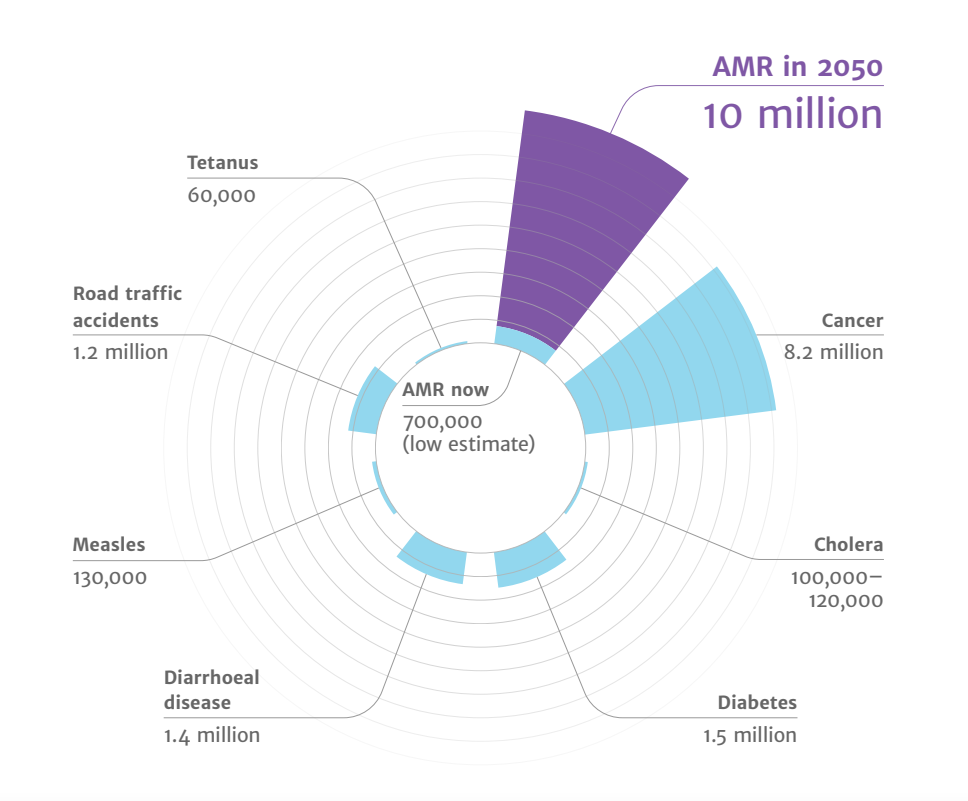
\includegraphics{images/AMR_deaths_2050.png}

}

\caption{\label{fig-oneilreport}Projected deaths due to antimicrobial
resistance in 2050. Source: O'Neil Report.}

\end{figure}

\hypertarget{key-concepts-for-review}{%
\section{Key concepts for review}\label{key-concepts-for-review}}

\begin{itemize}
\tightlist
\item
  Concept 1
\item
  Concept 2
\item
  Concept 3
\end{itemize}

\hypertarget{lecture-slides}{%
\section{Lecture slides}\label{lecture-slides}}

\bookmarksetup{startatroot}

\hypertarget{antibiotic-testing-in-the-laboratory-1}{%
\chapter{Antibiotic testing in the
laboratory}\label{antibiotic-testing-in-the-laboratory-1}}

\bookmarksetup{startatroot}

\hypertarget{antibiotic-testing-in-the-laboratory-2}{%
\chapter{Antibiotic testing in the
laboratory}\label{antibiotic-testing-in-the-laboratory-2}}

\bookmarksetup{startatroot}

\hypertarget{antibiotic-testing-in-the-laboratory-3}{%
\chapter{Antibiotic testing in the
laboratory}\label{antibiotic-testing-in-the-laboratory-3}}

\bookmarksetup{startatroot}

\hypertarget{antibiotic-testing-in-the-laboratory-4}{%
\chapter{Antibiotic testing in the
laboratory}\label{antibiotic-testing-in-the-laboratory-4}}

\bookmarksetup{startatroot}

\hypertarget{antibiotic-testing-in-the-laboratory-5}{%
\chapter{Antibiotic testing in the
laboratory}\label{antibiotic-testing-in-the-laboratory-5}}

\bookmarksetup{startatroot}

\hypertarget{antibiotic-testing-in-the-laboratory-6}{%
\chapter{Antibiotic testing in the
laboratory}\label{antibiotic-testing-in-the-laboratory-6}}

\bookmarksetup{startatroot}

\hypertarget{antibiotic-testing-in-the-laboratory-7}{%
\chapter{Antibiotic testing in the
laboratory}\label{antibiotic-testing-in-the-laboratory-7}}

\bookmarksetup{startatroot}

\hypertarget{antibiotic-testing-in-the-laboratory-8}{%
\chapter{Antibiotic testing in the
laboratory}\label{antibiotic-testing-in-the-laboratory-8}}

\bookmarksetup{startatroot}

\hypertarget{antibiotic-testing-in-the-laboratory-9}{%
\chapter{Antibiotic testing in the
laboratory}\label{antibiotic-testing-in-the-laboratory-9}}

\bookmarksetup{startatroot}

\hypertarget{antibiotic-testing-in-the-laboratory-10}{%
\chapter{Antibiotic testing in the
laboratory}\label{antibiotic-testing-in-the-laboratory-10}}

\bookmarksetup{startatroot}

\hypertarget{antibiotic-testing-in-the-laboratory-11}{%
\chapter{Antibiotic testing in the
laboratory}\label{antibiotic-testing-in-the-laboratory-11}}

\bookmarksetup{startatroot}

\hypertarget{antibiotic-testing-in-the-laboratory-12}{%
\chapter{Antibiotic testing in the
laboratory}\label{antibiotic-testing-in-the-laboratory-12}}

\bookmarksetup{startatroot}

\hypertarget{antibiotic-testing-in-the-laboratory-13}{%
\chapter{Antibiotic testing in the
laboratory}\label{antibiotic-testing-in-the-laboratory-13}}

\bookmarksetup{startatroot}

\hypertarget{antibiotic-testing-in-the-laboratory-14}{%
\chapter{Antibiotic testing in the
laboratory}\label{antibiotic-testing-in-the-laboratory-14}}

\bookmarksetup{startatroot}

\hypertarget{antibiotic-testing-in-the-laboratory-15}{%
\chapter{Antibiotic testing in the
laboratory}\label{antibiotic-testing-in-the-laboratory-15}}

\bookmarksetup{startatroot}

\hypertarget{summary}{%
\chapter{Summary}\label{summary}}

In summary, this book has no content whatsoever.

\begin{Shaded}
\begin{Highlighting}[]
\DecValTok{1} \SpecialCharTok{+} \DecValTok{1}
\end{Highlighting}
\end{Shaded}

\begin{verbatim}
[1] 2
\end{verbatim}

\bookmarksetup{startatroot}

\hypertarget{references}{%
\chapter*{References}\label{references}}
\addcontentsline{toc}{chapter}{References}

\markboth{References}{References}

\hypertarget{refs}{}
\begin{CSLReferences}{1}{0}
\leavevmode\vadjust pre{\hypertarget{ref-bush2010}{}}%
Bush, Karen, and George A. Jacoby. 2010. {``Updated Functional
Classification of β-Lactamases.''} \emph{Antimicrobial Agents and
Chemotherapy} 54 (3): 969--76.
\url{https://doi.org/10.1128/AAC.01009-09}.

\leavevmode\vadjust pre{\hypertarget{ref-davies_davies10}{}}%
Davies, Julian, and Dorothy Davies. 2010. {``Origins and {Evolution} of
{Antibiotic Resistance}.''} \emph{Microbiology and Molecular Biology
Reviews : MMBR} 74 (3): 417--33.
\url{https://doi.org/10.1128/MMBR.00016-10}.

\leavevmode\vadjust pre{\hypertarget{ref-holmes2016}{}}%
Holmes, Alison H, Luke S P Moore, Arnfinn Sundsfjord, Martin Steinbakk,
Sadie Regmi, Abhilasha Karkey, Philippe J Guerin, and Laura J V Piddock.
2016. {``Understanding the Mechanisms and Drivers of Antimicrobial
Resistance.''} \emph{The Lancet} 387 (10014): 176--87.
\url{https://doi.org/10.1016/S0140-6736(15)00473-0}.

\leavevmode\vadjust pre{\hypertarget{ref-kadri2018}{}}%
Kadri, Sameer S, Jennifer Adjemian, Yi Ling Lai, Alicen B Spaulding,
Emily Ricotta, D Rebecca Prevots, Tara N Palmore, et al. 2018.
{``Difficult-to-Treat Resistance in Gram-Negative Bacteremia at 173 US
Hospitals: Retrospective Cohort Analysis of Prevalence, Predictors, and
Outcome of Resistance to All First-Line Agents.''} \emph{Clinical
Infectious Diseases: An Official Publication of the Infectious Diseases
Society of America} 67 (12): 18031814.
\url{https://doi.org/10.1093/cid/ciy378}.

\leavevmode\vadjust pre{\hypertarget{ref-magiorakos2012}{}}%
Magiorakos, A-P, A Srinivasan, R B Carey, Y Carmeli, M E Falagas, C G
Giske, S Harbarth, et al. 2012. {``Multidrug-Resistant, Extensively
Drug-Resistant and Pandrug-Resistant Bacteria: An International Expert
Proposal for Interim Standard Definitions for Acquired Resistance.''}
\emph{Clinical Microbiology and Infection: The Official Publication of
the European Society of Clinical Microbiology and Infectious Diseases}
18 (3): 268281.
\url{http://onlinelibrary.wiley.com/doi/10.1111/j.1469-0691.2011.03570.x/pdf}.

\leavevmode\vadjust pre{\hypertarget{ref-verma_singh08}{}}%
Verma, Sheetal, and S. P. Singh. 2008. {``Current and Future Status of
Herbal Medicines.''} \emph{Veterinary World} 1 (11): 347.

\leavevmode\vadjust pre{\hypertarget{ref-wainwright89}{}}%
Wainwright, Milton. 1989. {``Moulds in Ancient and More Recent
Medicine.''} \emph{Mycologist} 3 (1): 21--23.

\end{CSLReferences}



\end{document}
